

%% Physics 101 Sample Test Questions by Dr. James Pierce
%%------------------------------------------------------------


%% JP's Physics 101 Test Bank 1
%%--------------------------------------------------

%% Topic: Equilibrium
\element{jpierce}{
\begin{question}{pt101tb1-Q01}
    When a ball is tossed straight up, it momentarily comes to a stop at the top of its path.
    Is it in equilibrium during this brief moment?
    \begin{choices}
        \wrongchoice{No, because it is weightless.}
        \wrongchoice{Yes, because there are no net forces acting on it.}
      \correctchoice{No, because its motion is changing.}
        \wrongchoice{Yes, because it is not moving.}
        \wrongchoice{Yes, because it has no inertia.}
    \end{choices}
\end{question}
}

\element{jpierce}{
\begin{question}{pt101tb1-Q02}
    A hockey puck slides across the ice at a constant speed.
    Is it in equilibrium?
    \begin{choices}
        \wrongchoice{No, because friction is slowing it down.}
        \wrongchoice{No, because it is moving.}
        \wrongchoice{No, because it has inertia.}
      \correctchoice{Yes, because there are no net forces acting on it.}
        \wrongchoice{Yes, because the ice exerts no forces on it.}
    \end{choices}
\end{question}
}

\element{jpierce}{
\begin{question}{pt101tb1-Q03}
    A book is at rest on top of a table.
    Which of the following is correct?
    \begin{choices}
        \wrongchoice{There is no force acting on the book.}
      \correctchoice{The book is in equilibrium.}
        \wrongchoice{The inertia of the book is equal to the inertia of the table.}
        \wrongchoice{There is no force acting on the table.}
        \wrongchoice{The book has no inertia.}
    \end{choices}
\end{question}
}

\element{jpierce}{
\begin{question}{pt101tb1-Q04}
    A parachutist falls toward the Earth's surface at a constant speed.
    How do the weight of the parachutist and the drag force on the parachute compare?
    \begin{choices}
        \wrongchoice{There is no connection between the drag force and the weight of the parachutist.}
        \wrongchoice{The drag force must be significantly less than the weight of the parachutist.}
        \wrongchoice{The drag force must be significantly greater than the weight of the parachutist.}
        \wrongchoice{This problem is impossible---a parachutist cannot fall at a constant speed.}
      \correctchoice{The drag force must be equal to the weight of the parachutist.}
    \end{choices}
\end{question}
}

\element{jpierce}{
\begin{question}{pt101tb1-Q05}
    Having made a slight miscalculation,
        Tarzan the ape man hangs motionless on a vertical grapevine suspended
        from a tall tree in the depths of the jungle.
    Which of the following is correct?
    \begin{choices}
        \wrongchoice{There is no tension in the grapevine.}
      \correctchoice{Tarzan is in equilibrium.}
        \wrongchoice{Tarzan has no inertia.}
        \wrongchoice{There are no forces acting on Tarzan.}
        \wrongchoice{Tarzan has no weight.}
    \end{choices}
\end{question}
}

\element{jpierce}{
\begin{question}{pt101tb1-Q06}
    A firefighter slides down a pole at a constant speed.
    How do the weight of the firefighter and the force of friction
        between the firefighter and the pole compare?
    \begin{choices}
        \wrongchoice{This problem is impossible---a firefighter cannot slide at a constant speed.}
        \wrongchoice{The frictional force must be significantly less than the weight of the firefighter.}
        \wrongchoice{There is no connection between the frictional force and the weight of the firefighter.}
      \correctchoice{The frictional force must be equal to the weight of the firefighter.}
        \wrongchoice{The frictional force must be significantly greater than the weight of the firefighter.}
    \end{choices}
\end{question}
}

\element{jpierce}{
\begin{question}{pt101tb1-Q07}
    A painter weighing \SI{750}{\newton} stands on a single board scaffold that
        is supported at each end by a vertical rope from above.
    If one rope has a tension of \SI{500}{\newton} and the other has a
        tension of \SI{350}{\newton}, what is the weight of the board?
    \begin{multicols}{3}
    \begin{choices}
        \wrongchoice{\SI{500}{\newton}}
        \wrongchoice{\SI{250}{\newton}}
        \wrongchoice{\SI{600}{\newton}}
        \wrongchoice{\SI{850}{\newton}}
      \correctchoice{\SI{100}{\newton}}
    \end{choices}
    \end{multicols}
\end{question}
}

\element{jpierce}{
\begin{question}{pt101tb1-Q08}
    A painter weighing \SI{700}{\newton} stands on a single board scaffold that
        is supported at each end by a vertical rope from above.
    If one rope has a tension of \SI{550}{\newton} and the other has a
        tension of \SI{400}{\newton}, what is the weight of the board?
    \begin{multicols}{3}
    \begin{choices}
        \wrongchoice{\SI{550}{\newton}}
        \wrongchoice{\SI{300}{\newton}}
        \wrongchoice{\SI{350}{\newton}}
        \wrongchoice{\SI{150}{\newton}}
      \correctchoice{\SI{250}{\newton}}
    \end{choices}
    \end{multicols}
\end{question}
}

\element{jpierce}{
\begin{question}{pt101tb1-Q09}
    A painter weighing \SI{800}{\newton} stands on a single board scaffold that
        is supported at each end by a vertical rope from above.
    If one rope has a tension of 550 newtons and the other has a
        tension of \SI{450}{\newton}, what is the weight of the board?
    \begin{multicols}{3}
    \begin{choices}
        \wrongchoice{\SI{250}{\newton}}
        \wrongchoice{\SI{100}{\newton}}
      \correctchoice{\SI{200}{\newton}}
        \wrongchoice{\SI{350}{\newton}}
        \wrongchoice{\SI{150}{\newton}}
    \end{choices}
    \end{multicols}
\end{question}
}

%% Topic: Inertia
\element{jpierce}{
\begin{question}{pt101tb1-Q10}
    The property of a moving object to continue moving is what Galileo called
    \begin{multicols}{2}
    \begin{choices}
        \wrongchoice{acceleration.}
        \wrongchoice{speed.}
        \wrongchoice{direction.}
        \wrongchoice{velocity.}
      \correctchoice{inertia.}
    \end{choices}
    \end{multicols}
\end{question}
}

\element{jpierce}{
\begin{question}{pt101tb1-Q11}
    The tendency of objects to resist changes in their motion is called
    \begin{multicols}{2}
    \begin{choices}
      \correctchoice{inertia.}
        \wrongchoice{velocity.}
        \wrongchoice{acceleration.}
        \wrongchoice{speed.}
        \wrongchoice{direction.}
    \end{choices}
    \end{multicols}
\end{question}
}

\element{jpierce}{
\begin{question}{pt101tb1-Q12}
    An automobile with relatively little inertia should
    \begin{choices}
      \correctchoice{get fairly good gas mileage.}
        \wrongchoice{be difficult to brake to a stop.}
        \wrongchoice{have room for lots of passengers.}
        \wrongchoice{be painted a light color, such as white.}
        \wrongchoice{need a big engine.}
    \end{choices}
\end{question}
}

\element{jpierce}{
\begin{question}{pt101tb1-Q13}
    Which of the following has the least amount of inertia?
    \begin{choices}
        \wrongchoice{a helicopter}
      \correctchoice{the wings of a hummingbird}
        \wrongchoice{your little finger}
        \wrongchoice{a bowling ball}
        \wrongchoice{the feet of an elephant}
    \end{choices}
\end{question}
}

%% Topic: Newtons first law
\element{jpierce}{
\begin{question}{pt101tb1-Q14}
    In the absence of an external net force, an object at rest remains at rest,
        and a body in motion moves in a straight line at constant speed. 
    This is a statement of:
    \begin{choices}
        \wrongchoice{Newton's Fourth Law of Motion.}
        \wrongchoice{Newton's Third Law of Motion.}
      \correctchoice{Newton's First Law of Motion.}
        \wrongchoice{Newton's Law of Gravity.}
        \wrongchoice{Newton's Second Law of Motion.}
    \end{choices}
\end{question}
}

\element{jpierce}{
\begin{question}{pt101tb1-Q15}
    A hockey puck sliding across the ice toward the goal is a good illustration of:
    \begin{choices}
        \wrongchoice{Newton's Second Law of Motion.}
      \correctchoice{Newton's First Law of Motion.}
        \wrongchoice{Newton's Fourth Law of Motion.}
        \wrongchoice{Newton's Law of Gravity}
        \wrongchoice{Newton's Third Law of Motion.}
    \end{choices}
\end{question}
}

\element{jpierce}{
\begin{question}{pt101tb1-Q16}
    According to Newton's First Law of Motion,
    \begin{choices}
      \correctchoice{an object in motion moves in a straight line unless acted upon by a net force.}
        \wrongchoice{an object at rest eventually begins to move.}
        \wrongchoice{an object in motion moves in a parabolic trajectory unless acted upon by a net force.}
        \wrongchoice{an object in motion eventually comes to a halt.}
        \wrongchoice{an object at rest always remains at rest.}
    \end{choices}
\end{question}
}

\element{jpierce}{
\begin{question}{pt101tb1-Q17}
    According to Newton's First Law of Motion,
    \begin{choices}
      \correctchoice{an object at rest remains at rest unless acted upon by a net force.}
        \wrongchoice{an object in motion moves in a parabolic trajectory unless acted upon by a net force.}
        \wrongchoice{an object at rest always remains at rest.}
        \wrongchoice{an object at rest eventually begins to move.}
        \wrongchoice{an object in motion eventually comes to a halt.}
    \end{choices}
\end{question}
}

%% Topic: Acc/Vel
\element{jpierce}{
\begin{question}{pt101tb1-Q18}
    \rule[-0.1pt]{4em}{0.1pt} is the rate of change of velocity due to a change in \rule[-0.1pt]{4em}{0.1pt}.
    \begin{choices}
        \wrongchoice{Direction; acceleration and/or speed}
        \wrongchoice{Speed; direction and/or acceleration}
        \wrongchoice{Time; the speed of light}
        \wrongchoice{Mass; inertia}
      \correctchoice{Acceleration; speed and/or direction}
    \end{choices}
\end{question}
}

\element{jpierce}{
\begin{question}{pt101tb1-Q19}
    Acceleration is the rate of change of \rule[-0.1pt]{4em}{0.1pt} due to a change in \rule[-0.1pt]{4em}{0.1pt}.
    \begin{choices}
        \wrongchoice{direction; velocity and/or speed}
        \wrongchoice{time; the speed of light}
        \wrongchoice{speed; direction and/or velocity}
      \correctchoice{velocity; speed and/or direction}
        \wrongchoice{mass; inertia}
    \end{choices}
\end{question}
}

\element{jpierce}{
\begin{question}{pt101tb1-Q20}
    Which of the following best expresses the relation between velocity and acceleration?
    \begin{choices}
        \wrongchoice{An object with zero acceleration must have zero velocity.}
        \wrongchoice{An object with zero acceleration must have non-zero velocity.}
      \correctchoice{The instantaneous acceleration and velocity of an object are independent of each other.}
        \wrongchoice{An object with non-zero acceleration must have zero velocity.}
        \wrongchoice{An object with non-zero acceleration must have non-zero velocity.}
    \end{choices}
\end{question}
}

\element{jpierce}{
\begin{question}{pt101tb1-Q21}
    If the acceleration of a car is directed toward the east,
        the velocity of the car
    \begin{choices}
        \wrongchoice{cannot be directed toward the north or the south.}
        \wrongchoice{must be directed toward the east.}
      \correctchoice{may have any direction.}
        \wrongchoice{must be zero.}
        \wrongchoice{must be directed toward the west.}
    \end{choices}
\end{question}
}

\element{jpierce}{
\begin{question}{pt101tb1-Q22}
    If an object is moving,
        then the magnitude of its \rule[-0.1pt]{4em}{0.1pt} cannot be zero.
    \begin{choices}
        \wrongchoice{speed}
        \wrongchoice{velocity}
        \wrongchoice{acceleration}
      \correctchoice{speed and velocity}
        \wrongchoice{speed, velocity and acceleration}
    \end{choices}
\end{question}
}

\element{jpierce}{
\begin{question}{pt101tb1-Q23}
    \rule[-0.1pt]{4em}{0.1pt} is the rate of change of \rule[-0.1pt]{4em}{0.1pt} due
        to a change in speed and/or direction.
    \begin{choices}
        \wrongchoice{Velocity; inertia}
        \wrongchoice{Velocity; acceleration}
        \wrongchoice{Mass; inertia}
        \wrongchoice{Inertia; mass}
      \correctchoice{Acceleration; velocity}
    \end{choices}
\end{question}
}

\newcommand{\jpierceTBOneQTwentyFourX}{
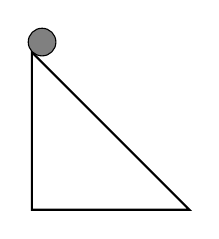
\begin{tikzpicture}
    \draw[thick] (0,0) -- (0,2) -- (2,0) -- cycle;
    \node[circle,fill=white!50!black,draw,minimum size=1em,anchor=south west] at (0,2) {};
\end{tikzpicture}
}

\newcommand{\jpierceTBOneQTwentyFourY}{
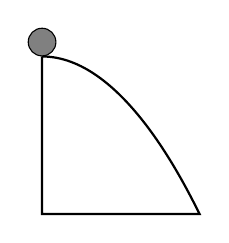
\begin{tikzpicture}
    \draw[thick] (0,2) -- (0,0) -- (2,0) parabola bend (0,2) (0,2);
    \node[circle,fill=white!50!black,draw,minimum size=1em,anchor=south] at (0,2) {};
\end{tikzpicture}
}

\newcommand{\jpierceTBOneQTwentyFourZ}{
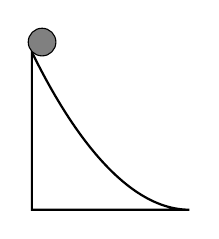
\begin{tikzpicture}
    \draw[thick] (2,0) -- (0,0) -- (0,2) parabola bend (2,0) (2,0);
    \node[circle,fill=white!50!black,draw,minimum size=1em,anchor=south west] at (0,2) {};
\end{tikzpicture}
}


%% Topic: Acc/Vel -3P
\element{jpierce}{
\begin{questionmult}{pt101tb1-Q24}
    In each case shown, a ball is released from rest and then rolls down the slope.
    In which case(s) does the ball roll with a constant acceleration?
    \begin{multicols}{2}
    \begin{choices}
        \AMCboxDimensions{down=-0.9cm}
      \correctchoice{\jpierceTBOneQTwentyFourX}
        \wrongchoice{\jpierceTBOneQTwentyFourY}
        \wrongchoice{\jpierceTBOneQTwentyFourZ}
        %\wrongchoice{None of these.}
        %\wrongchoice{$X$, $Y$ and $Z$}
        %\wrongchoice{$Z$}
        %\correctchoice{$X$}
        %\wrongchoice{$Y$}
    \end{choices}
    \end{multicols}
\end{questionmult}
}

\element{jpierce}{
\begin{questionmult}{pt101tb1-Q25}
    In each case shown, a ball is released from rest and then rolls down the slope.
    In which case(s) does the ball roll with a constant speed?
    \begin{multicols}{2}
    \begin{choices}
        \AMCboxDimensions{down=-0.9cm}
        \wrongchoice{\jpierceTBOneQTwentyFourX}
        \wrongchoice{\jpierceTBOneQTwentyFourY}
        \wrongchoice{\jpierceTBOneQTwentyFourZ}
        %\wrongchoice{$X$, $Y$ and $Z$}
        %\wrongchoice{$Y$}
        %\wrongchoice{$X$}
        %\wrongchoice{$Z$}
        %\correctchoice{None of these.}
    \end{choices}
    \end{multicols}
\end{questionmult}
}

\element{jpierce}{
\begin{questionmult}{pt101tb1-Q26}
    In each case shown, a ball is released from rest and then rolls down the slope.
    In which case(s) does the downward acceleration of the ball increase with time?
    \begin{multicols}{2}
    \begin{choices}
        \AMCboxDimensions{down=-0.9cm}
        \wrongchoice{\jpierceTBOneQTwentyFourX}
      \correctchoice{\jpierceTBOneQTwentyFourY}
        \wrongchoice{\jpierceTBOneQTwentyFourZ}
        %\wrongchoice{$Z$}
        %\wrongchoice{$X$, $Y$ and $Z$}
        %\wrongchoice{None of these.}
        %\wrongchoice{$X$}
        %\correctchoice{$Y$}
    \end{choices}
    \end{multicols}
\end{questionmult}
}

\element{jpierce}{
\begin{questionmult}{pt101tb1-Q27}
    In each case shown, a ball is released from rest and then rolls down the slope.
    In which case(s) does the downward acceleration of the ball decrease with time?
    \begin{multicols}{2}
    \begin{choices}
        \AMCboxDimensions{down=-0.9cm}
        \wrongchoice{\jpierceTBOneQTwentyFourX}
        \wrongchoice{\jpierceTBOneQTwentyFourY}
      \correctchoice{\jpierceTBOneQTwentyFourZ}
        %\wrongchoice{$X$}
        %\wrongchoice{$X$, $Y$ and $Z$}
        %\correctchoice{$Z$}
        %\wrongchoice{None of these.}
        %\wrongchoice{$Y$}
    \end{choices}
    \end{multicols}
\end{questionmult}
}

\element{jpierce}{
\begin{questionmult}{pt101tb1-Q28}
    In each case shown, a ball is released from rest and then rolls down the slope.
    In which case(s) does the speed of the ball increase with time?
    \begin{multicols}{2}
    \begin{choices}
        \AMCboxDimensions{down=-0.9cm}
      \correctchoice{\jpierceTBOneQTwentyFourX}
      \correctchoice{\jpierceTBOneQTwentyFourY}
      \correctchoice{\jpierceTBOneQTwentyFourZ}
        %\wrongchoice{$Y$}
        %\correctchoice{$X$, $Y$ and $Z$}
        %\wrongchoice{$X$}
        %\wrongchoice{None of these.}
        %\wrongchoice{$Z$}
    \end{choices}
    \end{multicols}
\end{questionmult}
}

\element{jpierce}{
\begin{questionmult}{pt101tb1-Q29}
    In each case shown, a ball is released from rest and then rolls down the slope.
    In which case(s) does the speed of the ball decrease with time?
    \begin{multicols}{2}
    \begin{choices}
        \AMCboxDimensions{down=-0.9cm}
        \wrongchoice{\jpierceTBOneQTwentyFourX}
        \wrongchoice{\jpierceTBOneQTwentyFourY}
        \wrongchoice{\jpierceTBOneQTwentyFourZ}
        %\wrongchoice{$X$, $Y$ and $Z$}
        %\wrongchoice{$X$}
        %\correctchoice{None of these.}
        %\wrongchoice{$Y$}
        %\wrongchoice{$Z$}
    \end{choices}
    \end{multicols}
\end{questionmult}
}

\element{jpierce}{
\begin{questionmult}{pt101tb1-Q30}
    In each case shown, a ball is released from rest and then rolls down the slope.
    In which case(s) does the ball reach the bottom in the shortest time?
    \begin{multicols}{2}
    \begin{choices}
        \AMCboxDimensions{down=-0.9cm}
        \wrongchoice{\jpierceTBOneQTwentyFourX}
        \wrongchoice{\jpierceTBOneQTwentyFourY}
      \correctchoice{\jpierceTBOneQTwentyFourZ}
        %\wrongchoice{$Y$}
        %\wrongchoice{$X$}
        %\correctchoice{$Z$}
        %\wrongchoice{both $Y$ and $Z$}
        %\wrongchoice{all three require the same time}
    \end{choices}
    \end{multicols}
\end{questionmult}
}

\element{jpierce}{
\begin{questionmult}{pt101tb1-Q31}
    In each case shown, a ball is released from rest and then rolls down the slope.
    In which case(s) does the ball require the longest time to reach the bottom?
    \begin{multicols}{2}
    \begin{choices}
        \AMCboxDimensions{down=-0.9cm}
        \wrongchoice{\jpierceTBOneQTwentyFourX}
      \correctchoice{\jpierceTBOneQTwentyFourY}
        \wrongchoice{\jpierceTBOneQTwentyFourZ}
        %\correctchoice{$Y$}
        %\wrongchoice{all three require the same time}
        %\wrongchoice{$X$}
        %\wrongchoice{both $Y$ and $Z$}
        %\wrongchoice{$Z$}
    \end{choices}
    \end{multicols}
\end{questionmult}
}


%% Topic: Acceleration
\element{jpierce}{
\begin{question}{pt101tb1-Q32}
    A car traveling on a circular track at \SI{50}{\kilo\meter\per\hour}
    \begin{choices}
      \correctchoice{is accelerating but has a constant speed.}
        \wrongchoice{has a changing speed but a constant velocity.}
        \wrongchoice{has a constant velocity but no acceleration.}
        \wrongchoice{is accelerating but has a constant velocity.}
        \wrongchoice{has a constant speed but no acceleration.}
    \end{choices}
\end{question}
}

\element{jpierce}{
\begin{question}{pt101tb1-Q33}
    When a car is accelerating, it must be:
    \begin{choices}
        \wrongchoice{changing its speed.}
        \wrongchoice{changing its color.}
      \correctchoice{changing its speed or its direction.}
        \wrongchoice{changing its position.}
        \wrongchoice{changing its direction.}
    \end{choices}
\end{question}
}

\element{jpierce}{
\begin{question}{pt101tb1-Q34}
    When a car is accelerating, it must be
    \begin{choices}
        \wrongchoice{changing its direction.}
        \wrongchoice{changing its position.}
        \wrongchoice{changing its shape.}
      \correctchoice{changing its velocity.}
        \wrongchoice{changing its speed.}
    \end{choices}
\end{question}
}

\element{jpierce}{
\begin{question}{pt101tb1-Q35}
    A car on a straight track went from \SI{0}{\mile\per\hour} to 
        \SI{60}{\mile\per\hour} in \SI{10}{\second}.
    Its \rule[-0.1pt]{4em}{0.1pt} was \SI{6}{\mile\per\hour\per\second}.
    \begin{choices}
      \correctchoice{acceleration}
        \wrongchoice{instantaneous velocity}
        \wrongchoice{free fall velocity}
        \wrongchoice{velocity}
        \wrongchoice{average speed}
    \end{choices}
\end{question}
}

\element{jpierce}{
\begin{question}{pt101tb1-Q36}
    A car travels for \SI{10}{\second} on a straight track at
        a constant speed of \SI{40}{\meter\per\second}.
    What is its acceleration during this period?
    \begin{multicols}{3}
    \begin{choices}
        \wrongchoice{\SI{40}{\meter\per\second}}
        \wrongchoice{\SI{10}{\meter\per\second\squared}}
      \correctchoice{\SI{0}{\meter\per\second\squared}}
        \wrongchoice{\SI{40}{\meter\per\second\squared}}
        \wrongchoice{\SI{4}{\meter\per\second\squared}}
    \end{choices}
    \end{multicols}
\end{question}
}

\element{jpierce}{
\begin{question}{pt101tb1-Q37}
    A car on a straight track is traveling at \SI{20}{\meter\per\second}.
    If the car accelerates for \SI{3}{\second} at \SI{5}{\meter\per\second\squared},
        what will be the car's speed at the end of the acceleration?
    \begin{multicols}{3}
    \begin{choices}
        \wrongchoice{\SI{15}{\meter\per\second}}
        \wrongchoice{\SI{65}{\meter\per\second}}
      \correctchoice{\SI{35}{\meter\per\second}}
        \wrongchoice{\SI{28}{\meter\per\second}}
        \wrongchoice{\SI{25}{\meter\per\second}}
    \end{choices}
    \end{multicols}
\end{question}
}

\element{jpierce}{
\begin{question}{pt101tb1-Q38}
    A car on a straight track is traveling at \SI{15}{\meter\per\second}.
    If the car accelerates for \SI{2}{\second} at \SI{5}{\meter\per\second\squared},
        what will be the car's speed at the end of the acceleration?
    \begin{multicols}{3}
    \begin{choices}
      \correctchoice{\SI{25}{\meter\per\second}}
        \wrongchoice{\SI{150}{\meter\per\second}}
        \wrongchoice{\SI{40}{\meter\per\second}}
        \wrongchoice{\SI{35}{\meter\per\second}}
        \wrongchoice{\SI{10}{\meter\per\second}}
    \end{choices}
    \end{multicols}
\end{question}
}

\element{jpierce}{
\begin{question}{pt101tb1-Q39}
    A car on a straight track is traveling at \SI{15}{\meter\per\second}.
    After the car decelerates for \SI{2}{\second} at \SI{5}{\meter\per\second\squared},
        what will be the car's new speed?
    \begin{multicols}{3}
    \begin{choices}
      \correctchoice{\SI{5}{\meter\per\second}}
        \wrongchoice{\SI{10}{\meter\per\second}}
        \wrongchoice{\SI{0}{\meter\per\second}}
        \wrongchoice{\SI{7}{\meter\per\second}}
        \wrongchoice{\SI{8}{\meter\per\second}}
    \end{choices}
    \end{multicols}
\end{question}
}

\element{jpierce}{
\begin{question}{pt101tb1-Q40}
    A car on a straight track is traveling at \SI{25}{\meter\per\second}.
    If the car accelerates for \SI{3}{\second} at \SI{5}{\meter\per\second\squared},
        what will be the car's speed at the end of the acceleration?
    \begin{multicols}{3}
    \begin{choices}
      \correctchoice{\SI{10}{\meter\per\second}}
        \wrongchoice{\SI{5}{\meter\per\second}}
        \wrongchoice{\SI{17}{\meter\per\second}}
        \wrongchoice{\SI{0}{\meter\per\second}}
        \wrongchoice{\SI{15}{\meter\per\second}}
    \end{choices}
    \end{multicols}
\end{question}
}

\element{jpierce}{
\begin{question}{pt101tb1-Q41}
    A car initially at rest accelerates in a straight line at \SI{3}{\meter\per\second\squared}. 
    What will be its speed after \SI{4}{\second}?
    \begin{multicols}{3}
    \begin{choices}
      \correctchoice{\SI{12}{\meter\per\second}}
        \wrongchoice{\SI{3}{\meter\per\second}}
        \wrongchoice{\SI{4}{\meter\per\second}}
        \wrongchoice{\SI{0}{\meter\per\second}}
        \wrongchoice{\SI{7}{\meter\per\second}}
    \end{choices}
    \end{multicols}
\end{question}
}

\element{jpierce}{
\begin{question}{pt101tb1-Q42}
    A car initially at rest accelerates in a straight line at \SI{3}{\meter\per\second\squared}.
    What will be its speed after \SI{2}{\second}?
    \begin{multicols}{3}
    \begin{choices}
        \wrongchoice{\SI{2}{\meter\per\second}}
      \correctchoice{\SI{6}{\meter\per\second}}
        \wrongchoice{\SI{0}{\meter\per\second}}
        \wrongchoice{\SI{5}{\meter\per\second}}
        \wrongchoice{\SI{3}{\meter\per\second}}
    \end{choices}
    \end{multicols}
\end{question}
}

%% Topic: Free Fall
\element{jpierce}{
\begin{question}{pt101tb1-Q43}
    If a bowling ball is dropped from a height of \SI{10}{\meter} above the ground,
        it will:
    \begin{choices}
        \wrongchoice{fall downward at a constant speed until it hits the ground.}
        \wrongchoice{rise slowly upwards at a constant speed until it hits the moon.}
        \wrongchoice{fall downward at a constant velocity until it hits the ground.}
        \wrongchoice{fall downward at an ever-decreasing speed until it hits the ground.}
      \correctchoice{fall downward at an ever-increasing speed until it hits the ground.}
    \end{choices}
\end{question}
}

\element{jpierce}{
\begin{question}{pt101tb1-Q44}
    A body in free fall in a vacuum:
    \begin{choices}
        \wrongchoice{will have the same average speed during each second of its fall.}
        \wrongchoice{will not be accelerated during its fall.}
      \correctchoice{will have the same acceleration during each second of its fall.}
        \wrongchoice{will drop the same distance during each second of its fall.}
        \wrongchoice{will have a constant velocity during each second of its fall.}
    \end{choices}
\end{question}
}

\element{jpierce}{
\begin{question}{pt101tb1-Q45}
    While experimenting with different bodies in free fall,
        Galileo found that when air resistance is small enough to be neglected,
    \begin{choices}
        \wrongchoice{large bodies accelerate more rapidly than small bodies.}
      \correctchoice{all bodies accelerate at the same rate.}
        \wrongchoice{light bodies accelerate more rapidly than heavy bodies.}
        \wrongchoice{heavy bodies accelerate more rapidly than light bodies.}
        \wrongchoice{small bodies accelerate more rapidly than large bodies.}
    \end{choices}
\end{question}
}

\element{jpierce}{
\begin{question}{pt101tb1-Q46}
    A baseball is thrown straight up with a speed of \SI{30}{\meter\per\second}.
    What is its acceleration immediately after its release?
    \begin{multicols}{2}
    \begin{choices}
        \wrongchoice{zero}
      \correctchoice{\SI{10}{\meter\per\second\squared} downward}
        \wrongchoice{\SI{15}{\meter\per\second} upward}
        \wrongchoice{\SI{30}{\meter\per\second\squared} downward}
        \wrongchoice{\SI{30}{\meter\per\second} upward}
    \end{choices}
    \end{multicols}
\end{question}
}

\element{jpierce}{
\begin{question}{pt101tb1-Q47}
    A baseball is thrown straight up with a speed of \SI{40}{\meter\per\second}.
    What is its acceleration one second after its release?
    \begin{multicols}{2}
    \begin{choices}
        \wrongchoice{\SI{30}{\meter\per\second\squared} upward}
        \wrongchoice{zero}
        \wrongchoice{\SI{20}{\meter\per\second\squared} downward}
      \correctchoice{\SI{10}{\meter\per\second\squared} downward}
        \wrongchoice{\SI{20}{\meter\per\second} upward}
    \end{choices}
    \end{multicols}
\end{question}
}

\element{jpierce}{
\begin{question}{pt101tb1-Q48}
    A baseball is thrown straight up with a speed of \SI{20}{\meter\per\second}.
    What is its acceleration two seconds after its release?
    \begin{multicols}{2}
    \begin{choices}
        \wrongchoice{\SI{10}{\meter\per\second\squared} upward}
      \correctchoice{\SI{10}{\meter\per\second\squared} downward}
        \wrongchoice{zero}
        \wrongchoice{\SI{20}{\meter\per\second} upward}
        \wrongchoice{\SI{20}{\meter\per\second\squared} downward}
    \end{choices}
    \end{multicols}
\end{question}
}

\element{jpierce}{
\begin{question}{pt101tb1-Q49}
    A baseball is thrown straight up at a speed of \SI{30}{\meter\per\second},
        then caught by the same player when it comes back down.
    What is the speed of the baseball the instant before it is caught?
    \begin{multicols}{2}
    \begin{choices}
        \wrongchoice{\SI{60}{\meter\per\second}}
        \wrongchoice{\SI{0}{\meter\per\second}}
      \correctchoice{\SI{30}{\meter\per\second}}
        \wrongchoice{\SI{15}{\meter\per\second}}
        \wrongchoice{\SI{90}{\meter\per\second}}
    \end{choices}
    \end{multicols}
\end{question}
}

\element{jpierce}{
\begin{question}{pt101tb1-Q50}
    A bowling ball at a height of \SI{20}{\meter} above the ground is falling
        vertically at a rate of \SI{10}{\meter\per\second}.
    Which of these best describes its fate?
    \begin{choices}
        \wrongchoice{It will hit the ground in more than two seconds at a speed less than \SI{10}{\meter\per\second}.}
      \correctchoice{It will hit the ground in less than two seconds at a speed greater than \SI{10}{\meter\per\second}.}
        \wrongchoice{It will hit the ground in exactly two seconds at a speed of \SI{10}{\meter\per\second}.}
        \wrongchoice{It will hit the ground in more than two seconds at a speed greater than \SI{10}{\meter\per\second}.}
        \wrongchoice{It will hit the ground in less than two seconds at a speed less than \SI{10}{\meter\per\second}.}
    \end{choices}
\end{question}
}

\element{jpierce}{
\begin{question}{pt101tb1-Q51}
    A bowling ball at a height of \SI{36}{\meter} above the ground is falling
        vertically at a rate of \SI{12}{\meter\per\second}. 
    Which of these best describes its fate?
    \begin{choices}
        \wrongchoice{It will hit the ground in more than three seconds at a speed greater than \SI{12}{\meter\per\second}.}
        \wrongchoice{It will hit the ground in less than three seconds at a speed less than \SI{12}{\meter\per\second}.}
        \wrongchoice{It will hit the ground in exactly three seconds at a speed of \SI{12}{\meter\per\second}.}
        \wrongchoice{It will hit the ground in more than three seconds at a speed less than \SI{12}{\meter\per\second}.}
      \correctchoice{It will hit the ground in less than three seconds at a speed greater than \SI{12}{\meter\per\second}.}
    \end{choices}
\end{question}
}

\element{jpierce}{
\begin{question}{pt101tb1-Q52}
    A bowling ball is dropped from rest from a height of \SI{50}{\meter}. 
    One second after its release, 
        the speed of the ball will be \rule[-0.1pt]{4em}{0.1pt} (neglecting air resistance).
    \begin{multicols}{3}
    \begin{choices}
      \correctchoice{\SI{10}{\meter\per\second}}
        \wrongchoice{\SI{100}{\meter\per\second}}
        \wrongchoice{\SI{5}{\meter\per\second}}
        \wrongchoice{\SI{20}{\meter\per\second}}
        \wrongchoice{\SI{0}{\meter\per\second}}
    \end{choices}
    \end{multicols}
\end{question}
}

\element{jpierce}{
\begin{question}{pt101tb1-Q53}
    During the first second after being released from rest,
        a free-falling ball will drop a distance of:
    \begin{multicols}{3}
    \begin{choices}
      \correctchoice{\SI{5}{\meter}}
        \wrongchoice{\SI{0.5}{\meter}}
        \wrongchoice{\SI{15}{\meter}}
        \wrongchoice{\SI{10}{\meter}}
        \wrongchoice{\SI{1}{\meter}}
    \end{choices}
    \end{multicols}
\end{question}
}

\element{jpierce}{
\begin{question}{pt101tb1-Q54}
    A person standing at the edge of a cliff \SI{30}{\meter} high throws one
        baseball upwards at \SI{20}{\meter\per\second} and then another baseball
        downwards at \SI{20}{\meter\per\second} such that both baseballs land
        at the base of the cliff at exactly the same time.
    How will the speeds of the two balls compare at the moment of impact
        (assuming air resistance is negligible)?
    \begin{choices}
      \correctchoice{Both balls will have essentially the same speed.}
        \wrongchoice{The `upward' ball will be moving faster because it fell from a greater height.}
        \wrongchoice{The `downward' ball will be moving faster because it did not have to change directions.}
        \wrongchoice{The `upward' ball will be moving faster because it had a longer time to accelerate.}
        \wrongchoice{The `downward' ball will be moving faster because it traveled a shorter distance.}
    \end{choices}
\end{question}
}

\element{jpierce}{
\begin{question}{pt101tb1-Q55}
    A bowling ball is dropped from rest from a height of \SI{60}{\meter}.
    Two seconds after its release, the speed of the ball will
        be \rule[-0.1pt]{4em}{0.1pt} (neglecting air resistance).
    \begin{multicols}{3}
    \begin{choices}
        \wrongchoice{\SI{10}{\meter\per\second}}
        \wrongchoice{\SI{0}{\meter\per\second}}
        \wrongchoice{\SI{40}{\meter\per\second}}
        \wrongchoice{\SI{5}{\meter\per\second}}
      \correctchoice{\SI{20}{\meter\per\second}}
    \end{choices}
    \end{multicols}
\end{question}
}

%% Topic: Speed
\element{jpierce}{
\begin{question}{pt101tb1-Q56}
    A train traveled a distance of \SI{90}{\kilo\meter} in \SI{2}{\hour}.
    It would be most correct to say that its \rule[-0.1pt]{4em}{0.1pt} was
        \SI{45}{\kilo\meter\per\hour}.
    \begin{choices}
      \correctchoice{average speed}
        \wrongchoice{acceleration}
        \wrongchoice{velocity}
        \wrongchoice{free fall velocity}
        \wrongchoice{instantaneous speed}
    \end{choices}
\end{question}
}

\element{jpierce}{
\begin{question}{pt101tb1-Q57}
    A car on a straight track accelerated uniformly from \SI{0}{\mile\per\hour}
        to \SI{60}{\mile\per\hour} in \SI{10}{\second}.
    Its \rule[-0.1pt]{4em}{0.1pt} was \SI{30}{\mile\per\hour}.
    \begin{choices}
        \wrongchoice{instantaneous velocity}
        \wrongchoice{velocity}
        \wrongchoice{free fall velocity}
        \wrongchoice{acceleration}
      \correctchoice{average speed}
    \end{choices}
\end{question}
}

\element{jpierce}{
\begin{question}{pt101tb1-Q58}
    A car on a straight track accelerated uniformly from \SI{0}{\mile\per\hour}
        to \SI{50}{\mile\per\hour} in \SI{20}{\second}.
    Its \rule[-0.1pt]{4em}{0.1pt} was \SI{25}{\mile\per\hour}.
    \begin{choices}
        \wrongchoice{acceleration}
        \wrongchoice{free fall velocity}
        \wrongchoice{instantaneous velocity}
      \correctchoice{average speed}
        \wrongchoice{velocity}
    \end{choices}
\end{question}
}

\element{jpierce}{
\begin{question}{pt101tb1-Q59}
    The speedometer in your car tells you the \rule[-0.1pt]{4em}{0.1pt} of your car.
    \begin{choices}
        \wrongchoice{average speed}
        \wrongchoice{inertia}
        \wrongchoice{acceleration}
        \wrongchoice{velocity}
      \correctchoice{instantaneous speed}
    \end{choices}
\end{question}
}

\element{jpierce}{
\begin{question}{pt101tb1-Q60}
    The cruise control on an automobile is designed to maintain
        the moving vehicle at a nearly constant
    \begin{multicols}{2}
    \begin{choices}
        \wrongchoice{inertia.}
        \wrongchoice{acceleration.}
        \wrongchoice{direction.}
      \correctchoice{speed.}
        \wrongchoice{velocity.}
    \end{choices}
    \end{multicols}
\end{question}
}

\element{jpierce}{
\begin{question}{pt101tb1-Q61}
    A train traveled a distance of \SI{100}{\kilo\meter} in \SI{2}{\hour}.
    Its average speed was:
    %\rule[-0.1pt]{4em}{0.1pt} \si{\kilo\meter\per\hour}:
    \begin{multicols}{3}
    \begin{choices}
        \wrongchoice{\SI{200}{\kilo\meter\per\hour}}
        \wrongchoice{\SI{75}{\kilo\meter\per\hour}}
        \wrongchoice{\SI{100}{\kilo\meter\per\hour}}
        \wrongchoice{\SI{2}{\kilo\meter\per\hour}}
      \correctchoice{\SI{50}{\kilo\meter\per\hour}}
    \end{choices}
    \end{multicols}
\end{question}
}

\element{jpierce}{
\begin{question}{pt101tb1-Q62}
    A train traveled a distance of \SI{180}{\kilo\meter} in \SI{5}{\hour}.
    Its average speed was:
    %\rule[-0.1pt]{4em}{0.1pt} \si{\kilo\meter\per\hour}:
    \begin{multicols}{3}
    \begin{choices}
      \correctchoice{\SI{36}{\kilo\meter\per\hour}}
        \wrongchoice{\SI{60}{\kilo\meter\per\hour}}
        \wrongchoice{\SI{30}{\kilo\meter\per\hour}}
        \wrongchoice{\SI{45}{\kilo\meter\per\hour}}
        \wrongchoice{\SI{90}{\kilo\meter\per\hour}}
    \end{choices}
    \end{multicols}
\end{question}
}

\element{jpierce}{
\begin{question}{pt101tb1-Q63}
    An airplane flew in a straight line for \SI{2}{\hour}
        at an average speed of \SI{300}{\kilo\meter\per\hour}.
    It traveled a distance of:
    %\rule[-0.1pt]{4em}{0.1pt} \si{\kilo\meter}:
    \begin{multicols}{3}
    \begin{choices}
        \wrongchoice{\SI{300}{\kilo\meter}}
      \correctchoice{\SI{600}{\kilo\meter}}
        \wrongchoice{\SI{150}{\kilo\meter}}
        \wrongchoice{\SI{500}{\kilo\meter}}
        \wrongchoice{\SI{400}{\kilo\meter}}
    \end{choices}
    \end{multicols}
\end{question}
}

\element{jpierce}{
\begin{question}{pt101tb1-Q64}
    An airplane flew in a straight line for \SI{2}{\hour} and traveled a distance of \SI{500}{\kilo\meter};
        its average speed was:
    %\rule[-0.1pt]{4em}{0.1pt} \si{\kilo\meter\per\hour}.
    \begin{multicols}{2}
    \begin{choices}
        \wrongchoice{\SI{500}{\kilo\meter\per\hour}}
      \correctchoice{\SI{250}{\kilo\meter\per\hour}}
        \wrongchoice{\SI{1000}{\kilo\meter\per\hour}}
        \wrongchoice{\SI{750}{\kilo\meter\per\hour}}
        \wrongchoice{\SI{100}{\kilo\meter\per\hour}}
    \end{choices}
    \end{multicols}
\end{question}
}

%% Topic: Velocity
\element{jpierce}{
\begin{question}{pt101tb1-Q65}
    To report the velocity of an object,
        we must specify both its \rule[-0.1pt]{4em}{0.1pt} and its \rule[-0.1pt]{4em}{0.1pt}.
    \begin{choices}
        \wrongchoice{mass; length}
        \wrongchoice{direction; mass}
      \correctchoice{speed; direction}
        \wrongchoice{length; acceleration}
        \wrongchoice{acceleration; speed}
    \end{choices}
\end{question}
}

\element{jpierce}{
\begin{question}{pt101tb1-Q66}
    To report the velocity of an object,
        we must specify both its speed and its \rule[-0.1pt]{4em}{0.1pt}.
    \begin{multicols}{2}
    \begin{choices}
        \wrongchoice{mass}
        \wrongchoice{position}
        \wrongchoice{acceleration}
        \wrongchoice{length}
      \correctchoice{direction}
    \end{choices}
    \end{multicols}
\end{question}
}

\element{jpierce}{
\begin{question}{pt101tb1-Q67}
    To report the velocity of an object,
        we must specify both its \rule[-0.1pt]{4em}{0.1pt} and its direction.
    \begin{multicols}{2}
    \begin{choices}
        \wrongchoice{acceleration}
        \wrongchoice{length}
        \wrongchoice{mass}
      \correctchoice{speed}
        \wrongchoice{position}
    \end{choices}
    \end{multicols}
\end{question}
}

\element{jpierce}{
\begin{question}{pt101tb1-Q68}
    To report the \rule[-0.1pt]{4em}{0.1pt} of an object,
        we must specify both its speed and its direction.
    \begin{multicols}{2}
    \begin{choices}
        \wrongchoice{acceleration}
        \wrongchoice{position}
        \wrongchoice{mass}
      \correctchoice{velocity}
        \wrongchoice{length}
    \end{choices}
    \end{multicols}
\end{question}
}

%% Topic: Proj Angle
\element{jpierce}{
\begin{question}{pt101tb1-Q69}
    Assuming level ground and no air resistance,
        a projectile fired at an angle of \ang{30} will have the same
        range as another projectile fired with the same speed at an angle of:
    \begin{multicols}{2}
    \begin{choices}[o]
        \wrongchoice{\ang{45}}
      \correctchoice{\ang{60}}
        \wrongchoice{\ang{90}}
        \wrongchoice{\ang{15}}
        \wrongchoice{none of these---each different projection angle produces a different range}
    \end{choices}
    \end{multicols}
\end{question}
}

\element{jpierce}{
\begin{question}{pt101tb1-Q70}
    Assuming level ground and no air resistance,
        a projectile fired at an angle of \ang{40} will have the same
        range as another projectile fired with the same speed at an angle of:
    \begin{multicols}{2}
    \begin{choices}[o]
      \correctchoice{\ang{50}}
        \wrongchoice{\ang{20}}
        \wrongchoice{\ang{80}}
        \wrongchoice{\ang{60}}
        \wrongchoice{none of these---each different projection angle produces a different range}
    \end{choices}
    \end{multicols}
\end{question}
}

\element{jpierce}{
\begin{question}{pt101tb1-Q71}
    Assuming level ground and no air resistance,
        a projectile fired at an angle of \ang{55} will have the same
        range as another projectile fired with the same speed at an angle of:
    \begin{multicols}{2}
    \begin{choices}[o]
        \wrongchoice{\ang{45}}
        \wrongchoice{\ang{15}}
        \wrongchoice{\ang{25}}
      \correctchoice{\ang{35}}
        \wrongchoice{none of these---each different projection angle produces a different range}
    \end{choices}
    \end{multicols}
\end{question}
}

\element{jpierce}{
\begin{question}{pt101tb1-Q72}
    Assuming level ground and no air resistance,
        a projectile fired at an angle of \ang{25} will have the same
        range as another projectile fired with the same speed at an angle of:
    \begin{multicols}{2}
    \begin{choices}[o]
      \correctchoice{\ang{65}}
        \wrongchoice{\ang{45}}
        \wrongchoice{\ang{55}}
        \wrongchoice{\ang{75}}
        \wrongchoice{none of these---each different projection angle produces a different range}
    \end{choices}
    \end{multicols}
\end{question}
}

\element{jpierce}{
\begin{question}{pt101tb1-Q73}
    Assuming level ground and no air resistance,
        a projectile fired at an angle of \ang{80} will have the same
        range as another projectile fired with the same speed at an angle of:
    \begin{multicols}{2}
    \begin{choices}[o]
      \correctchoice{\ang{10}}
        \wrongchoice{\ang{60}}
        \wrongchoice{\ang{20}}
        \wrongchoice{\ang{30}}
        \wrongchoice{none of these---each different projection angle produces a different range}
    \end{choices}
    \end{multicols}
\end{question}
}

\element{jpierce}{
\begin{question}{pt101tb1-Q74}
    Projectile $A$ is fired at an angle of \ang{50} above the horizontal;
        projectile $B$ is fired with the same speed at an angle of \ang{40}
        above the horizontal.
    Assuming level ground and negligible air resistance,
        which of the following is true?
    \begin{choices}
        \wrongchoice{$A$ will reach the same height and have a shorter range than $B$.}
        \wrongchoice{$A$ will reach a greater height and have a greater range than $B$.}
        \wrongchoice{$A$ will reach a greater height and have a shorter range than $B$.}
      \correctchoice{$A$ will reach a greater height and have the same range as $B$.}
        \wrongchoice{$A$ will reach the same height and have the same range as $B$.}
    \end{choices}
\end{question}
}

\element{jpierce}{
\begin{question}{pt101tb1-Q75}
    Projectile $A$ is fired at an angle of \ang{70} above the horizontal;
        projectile $B$ is fired with the same speed at an angle of \ang{20}
        above the horizontal.
    Assuming level ground and negligible air resistance,
        which of the following is true?
    \begin{choices}
      \correctchoice{$A$ will reach a greater height and have the same range as $B$.}
        \wrongchoice{$A$ will reach the same height and have a shorter range than $B$.}
        \wrongchoice{$A$ will reach a greater height and have a greater range than $B$.}
        \wrongchoice{$A$ will reach the same height and have the same range as $B$.}
        \wrongchoice{$A$ will reach a greater height and have a shorter range than $B$.}
    \end{choices}
\end{question}
}

\element{jpierce}{
\begin{question}{pt101tb1-Q76}
    Projectile $A$ is fired at an angle of \ang{70} above the horizontal;
        projectile $B$ is fired with the same speed at an angle of \ang{30}
        above the horizontal.
    Assuming level ground and negligible air resistance,
        which of the following is true?
    \begin{choices}
        \wrongchoice{$A$ will reach a greater height and have a greater range than $B$.}
        \wrongchoice{$A$ will reach a greater height and have the same range as $B$.}
        \wrongchoice{$A$ will reach the same height and have a shorter range than $B$.}
        \wrongchoice{$A$ will reach the same height and have the same range as $B$.}
      \correctchoice{$A$ will reach a greater height and have a shorter range than $B$.}
    \end{choices}
\end{question}
}

\element{jpierce}{
\begin{question}{pt101tb1-Q77}
    Projectile $A$ is fired at an angle of \ang{60} above the horizontal;
        projectile $B$ is fired with the same speed at an angle of \ang{20}
        above the horizontal.
    Assuming level ground and negligible air resistance,
        which of the following is true?
    \begin{choices}
        \wrongchoice{$A$ will reach the same height and have the same range as $B$.}
        \wrongchoice{$A$ will reach a greater height and have the same range as $B$.}
      \correctchoice{$A$ will reach a greater height and have a greater range than $B$.}
        \wrongchoice{$A$ will reach the same height and have a shorter range than $B$.}
        \wrongchoice{$A$ will reach a greater height and have a shorter range than $B$.}
    \end{choices}
\end{question}
}

\element{jpierce}{
\begin{question}{pt101tb1-Q78}
    Assuming level ground and no air resistance,
        the maximum range of a projectile will be obtained by firing it at an angle of:
    \begin{multicols}{3}
    \begin{choices}
        \wrongchoice{\ang{55}}
        \wrongchoice{\ang{75}}
      \correctchoice{\ang{45}}
        \wrongchoice{\ang{65}}
        \wrongchoice{\ang{85}}
    \end{choices}
    \end{multicols}
\end{question}
}

%% Topic: Projectile
\element{jpierce}{
\begin{question}{pt101tb1-Q79}
    In general, the maximum range of a projectile for a given initial speed
        is obtained with a projection angle of \rule[-0.1pt]{4em}{0.1pt} above
        the horizon (neglecting air resistance).
    \begin{multicols}{3}
    \begin{choices}
        \wrongchoice{\ang{30}}
        \wrongchoice{\ang{75}}
        \wrongchoice{\ang{90}}
      \correctchoice{\ang{45}}
        \wrongchoice{\ang{60}}
    \end{choices}
    \end{multicols}
\end{question}
}

\element{jpierce}{
\begin{question}{pt101tb1-Q80}
    In the absence of air resistance,
        the magnitude of the horizontal component of a projectile's velocity
    \begin{choices}
      \correctchoice{is constant until the projectile hits the ground.}
        \wrongchoice{increases with time until the projectile hits the ground.}
        \wrongchoice{decreases with time until the projectile hits the ground.}
        \wrongchoice{is equal to the magnitude of the vertical component of the projectile's velocity.}
        \wrongchoice{is equal to one half of the magnitude of the vertical component of the projectile's velocity.}
    \end{choices}
\end{question}
}

\element{jpierce}{
\begin{question}{pt101tb1-Q81}
    In the absence of air resistance,
        the magnitude of the vertical component of a projectile's velocity
    \begin{choices}
        \wrongchoice{is constant until the projectile hits the ground.}
        \wrongchoice{always increases with time until the projectile hits the ground.}
        \wrongchoice{always decreases with time until the projectile hits the ground.}
      \correctchoice{increases and/or decreases with time, due to the acceleration of gravity.}
        \wrongchoice{is equal to the magnitude of the horizontal component of the projectile's velocity.}
    \end{choices}
\end{question}
}

\element{jpierce}{
\begin{question}{pt101tb1-Q82}
    A ball is thrown at 30 m/s at an angle of \ang{60} above the horizontal.
    Which of the following statements about the ball's motion is true
        (assuming no air resistance)?
    \begin{choices}
        \wrongchoice{The magnitude of the velocity is constant until the ball strikes the ground.}
      \correctchoice{The horizontal component of the velocity is constant until the ball strikes the ground.}
        \wrongchoice{The vertical component of the velocity is constant until the ball strikes the ground.}
        \wrongchoice{The distance traveled by the ball each second is constant until the ball strikes the ground.}
        \wrongchoice{Both the horizontal and vertical components of the velocity will constantly change, due to gravity.}
    \end{choices}
\end{question}
}

\element{jpierce}{
\begin{question}{pt101tb1-Q83}
    When air resistance does not affect the motion of a projectile,
    \begin{choices}
        \wrongchoice{the horizontal and vertical components of its velocity will both change at the same rate.}
        \wrongchoice{the horizontal and vertical components of its velocity will both change, but at different rates.}
      \correctchoice{the vertical component of its velocity will change while the horizontal component remains constant.}
        \wrongchoice{the horizontal component of its velocity will change while the vertical component remains constant.}
        \wrongchoice{the horizontal and vertical components of its velocity will remain constant.}
    \end{choices}
\end{question}
}

\element{jpierce}{
\begin{question}{pt101tb1-Q84}
    In the absence of air resistance,
        the magnitude of the vertical component of a projectile's acceleration
    \begin{choices}
        \wrongchoice{always decreases with time until the projectile hits the ground.}
        \wrongchoice{increases and/or decreases with time, depending on the projectile's velocity.}
        \wrongchoice{is equal to the magnitude of the horizontal component of the projectile's acceleration.}
        \wrongchoice{always increases with time until the projectile hits the ground.}
      \correctchoice{is constant until the projectile hits the ground.}
    \end{choices}
\end{question}
}

\element{jpierce}{
\begin{question}{pt101tb1-Q85}
    In the absence of air resistance,
        the magnitude of the horizontal component of a projectile's acceleration
    \begin{choices}
        \wrongchoice{is equal to the magnitude of the vertical component of the projectile's acceleration.}
        \wrongchoice{increases with time until the projectile hits the ground.}
        \wrongchoice{is equal to one half of the magnitude of the vertical component of the projectile's acceleration.}
      \correctchoice{is constant until the projectile hits the ground.}
        \wrongchoice{decreases with time until the projectile hits the ground.}
    \end{choices}
\end{question}
}

\element{jpierce}{
\begin{question}{pt101tb1-Q86}
    A ball is thrown horizontally off the top of a high cliff.
    In the absence of air resistance,
        the vertical distance the ball travels in the first second
    \begin{choices}
        \wrongchoice{depends on the size of the ball---the bigger the ball, the greater the distance.}
        \wrongchoice{depends on the speed at which it was thrown---the higher the speed, the greater the distance.}
      \correctchoice{is always the same---about five meters.}
        \wrongchoice{depends on the size of the ball---the smaller the ball, the greater the distance.}
        \wrongchoice{depends on the speed at which it was thrown---the lower the speed, the greater the distance.}
    \end{choices}
\end{question}
}

\element{jpierce}{
\begin{question}{pt101tb1-Q87}
    A ball is thrown horizontally off the top of a high cliff.
    In the absence of air resistance,
        the horizontal distance the ball travels in the first second
    \begin{choices}
        \wrongchoice{is always the same---about five meters.}
        \wrongchoice{depends on the size of the ball---the bigger the ball, the greater the distance.}
        \wrongchoice{depends on the speed at which it was thrown---the lower the speed, the greater the distance.}
        \wrongchoice{depends on the size of the ball---the smaller the ball, the greater the distance.}
      \correctchoice{depends on the speed at which it was thrown---the higher the speed, the greater the distance.}
    \end{choices}
\end{question}
}

\element{jpierce}{
\begin{question}{pt101tb1-Q88}
    A ball is thrown horizontally with a speed of \SI{25}{\meter\per\second}
        from the top of a tower \SI{20}{\meter} high.
    Assuming level ground below and negligible air resistance,
        what will be the magnitude of the horizontal velocity
        component when the ball hits the ground?
    \begin{multicols}{3}
    \begin{choices}
        \wrongchoice{\SI{5}{\meter\per\second}}
        \wrongchoice{\SI{35}{\meter\per\second}}
        \wrongchoice{\SI{15}{\meter\per\second}}
        \wrongchoice{\SI{50}{\meter\per\second}}
      \correctchoice{\SI{25}{\meter\per\second}}
    \end{choices}
    \end{multicols}
\end{question}
}

\element{jpierce}{
\begin{question}{pt101tb1-Q89}
    A ball is thrown horizontally with a speed of \SI{15}{\meter\per\second}
        from the top of a tower \SI{20}{\meter} high.
    Assuming level ground below and negligible air resistance,
        what will be the magnitude of the horizontal velocity component
        when the ball hits the ground?
    \begin{multicols}{3}
    \begin{choices}
        \wrongchoice{\SI{5}{\meter\per\second}}
        \wrongchoice{\SI{35}{\meter\per\second}}
        \wrongchoice{\SI{25}{\meter\per\second}}
        \wrongchoice{\SI{50}{\meter\per\second}}
      \correctchoice{\SI{15}{\meter\per\second}}
    \end{choices}
    \end{multicols}
\end{question}
}

\element{jpierce}{
\begin{question}{pt101tb1-Q90}
    A ball is thrown horizontally with a speed of \SI{35}{\meter\per\second}
        from the top of a tower \SI{20}{\meter} high.
    Assuming level ground below and negligible air resistance,
        what will be the magnitude of the horizontal velocity component
        when the ball hits the ground?
    \begin{multicols}{3}
    \begin{choices}
        \wrongchoice{\SI{15}{\meter\per\second}}
      \correctchoice{\SI{35}{\meter\per\second}}
        \wrongchoice{\SI{25}{\meter\per\second}}
        \wrongchoice{\SI{5}{\meter\per\second}}
        \wrongchoice{\SI{50}{\meter\per\second}}
    \end{choices}
    \end{multicols}
\end{question}
}

\element{jpierce}{
\begin{question}{pt101tb1-Q91}
    A ball is thrown such that the vertical component of its motion is
        \SI{30}{\meter\per\second} upwards and the horizontal component
        of its motion is \SI{20}{\meter\per\second} to the north.
    How long will it be before the ball reaches its maximum height
        (neglecting air resistance)?
    \begin{multicols}{3}
    \begin{choices}
        \wrongchoice{about \SI{1.5}{\second}}
        \wrongchoice{about \SI{5}{\second}}
        \wrongchoice{about \SI{2}{\second}}
      \correctchoice{about \SI{3}{\second}}
        \wrongchoice{about \SI{10}{\second}}
    \end{choices}
    \end{multicols}
\end{question}
}

\element{jpierce}{
\begin{question}{pt101tb1-Q92}
    A ball is thrown such that the vertical component of its motion is
        \SI{30}{\meter\per\second} upwards and the horizontal component
        of its motion is \SI{20}{\meter\per\second} to the north.
    How long will it be before the ball hits the ground
        (assuming a level surface and neglecting air resistance)?
    \begin{multicols}{3}
    \begin{choices}
      \correctchoice{about \SI{6}{\second}}
        \wrongchoice{about \SI{3}{\second}}
        \wrongchoice{about \SI{4}{\second}}
        \wrongchoice{about \SI{8}{\second}}
        \wrongchoice{about \SI{10}{\second}}
    \end{choices}
    \end{multicols}
\end{question}
}

\element{jpierce}{
\begin{question}{pt101tb1-Q93}
    A ball is thrown horizontally with a speed of \SI{25}{\meter\per\second}
        from the top of a tower \SI{20}{\meter} high.
    Assuming level ground below and negligible air resistance,
        how much time will elapse before the ball hits the ground?
    \begin{multicols}{2}
    \begin{choices}
        \wrongchoice{about \SI{1}{\second}}
        \wrongchoice{about \SI{3}{\second}}
        \wrongchoice{about \SI{4}{\second}}
        \wrongchoice{about \SI{5}{\second}}
      \correctchoice{about \SI{2}{\second}}
    \end{choices}
    \end{multicols}
\end{question}
}

\element{jpierce}{
\begin{question}{pt101tb1-Q94}
    A ball is thrown horizontally with a speed of \SI{25}{\meter\per\second}
        from the top of a tower \SI{20}{\meter} high.
    Assuming level ground below and negligible air resistance,
        how far from the tower will the ball hit the ground?
    \begin{multicols}{3}
    \begin{choices}
        \wrongchoice{\SI{20}{\meter}}
        \wrongchoice{\SI{40}{\meter}}
        \wrongchoice{\SI{30}{\meter}}
        \wrongchoice{\SI{25}{\meter}}
      \correctchoice{\SI{50}{\meter}}
    \end{choices}
    \end{multicols}
\end{question}
}

\element{jpierce}{
\begin{question}{pt101tb1-Q95}
    A ball is thrown horizontally with a speed of \SI{25}{\meter\per\second}
        from the top of a tower \SI{20}{\meter} high.
    Assuming level ground below and negligible air resistance,
        what will be the magnitude of the vertical velocity
        component when the ball hits the ground?
    \begin{multicols}{3}
    \begin{choices}
        \wrongchoice{\SI{50}{\meter\per\second}}
        \wrongchoice{\SI{25}{\meter\per\second}}
        \wrongchoice{\SI{10}{\meter\per\second}}
        \wrongchoice{\SI{15}{\meter\per\second}}
      \correctchoice{\SI{20}{\meter\per\second}}
    \end{choices}
    \end{multicols}
\end{question}
}

%% Topic Trajectory
\element{jpierce}{
\begin{question}{pt101tb1-Q96}
    Which of these is the best description of the trajectory
        of a projectile shot at an angle of \ang{60} above the
        horizontal (neglecting air resistance)?
    \begin{choices}
        \wrongchoice{The projectile will gradually arc downward, following the curve of a circle.}
        \wrongchoice{The projectile will move upwards at a \ang{60} angle in a straight line at a gradually increasing speed until it stops and then falls straight down.}
        \wrongchoice{The projectile will move upwards at a \ang{60} angle in a straight line at a gradually diminishing speed until it stops and then falls straight down.}
      \correctchoice{The projectile will gradually arc downward, following the curve of a parabola.}
        \wrongchoice{The projectile will move upwards at a \ang{60} angle in a straight line at a constant speed until it stops and then falls straight down.}
    \end{choices}
\end{question}
}

\element{jpierce}{
\begin{question}{pt101tb1-Q97}
    Which of these is the best description of the trajectory of a
        projectile shot at an angle of \ang{30} above the horizontal
        (neglecting air resistance)?
    \begin{choices}
        \wrongchoice{The projectile will move upwards at a \ang{30} angle in a straight line at a gradually diminishing speed until it stops and then falls straight down.}
      \correctchoice{The projectile will gradually arc downward, following the curve of a parabola.}
        \wrongchoice{The projectile will gradually arc downward, following the curve of a circle.}
        \wrongchoice{The projectile will move upwards at a \ang{30} angle in a straight line at a gradually increasing speed until it stops and then falls straight down.}
        \wrongchoice{The projectile will move upwards at a \ang{30} angle in a straight line at a constant speed until it stops and then falls straight down.}
    \end{choices}
\end{question}
}

\element{jpierce}{
\begin{question}{pt101tb1-Q98}
    Which of these is the best description of the trajectory of a
        projectile shot at an angle of \ang{45} above the horizontal
        (neglecting air resistance)?
    \begin{choices}
      \correctchoice{The projectile will gradually arc downward, following the curve of a parabola.}
        \wrongchoice{The projectile will gradually arc downward, following the curve of a circle.}
        \wrongchoice{The projectile will move upwards at a \ang{45} angle in a straight line at a constant speed until it stops and then falls straight down.}
        \wrongchoice{The projectile will move upwards at a \ang{45} angle in a straight line at a gradually increasing speed until it stops and then falls straight down.}
        \wrongchoice{The projectile will move upwards at a \ang{45} angle in a straight line at a gradually diminishing speed until it stops and then falls straight down.}
    \end{choices}
\end{question}
}

\element{jpierce}{
\begin{question}{pt101tb1-Q99}
    Which of these is the best description of the trajectory of a
        projectile shot horizontally off a high cliff
        (neglecting air resistance)?
    \begin{choices}
        \wrongchoice{The projectile will move outwards in a straight line at a gradually diminishing speed until it stops and then falls straight down.}
        \wrongchoice{The projectile will move outwards in a straight line at a gradually increasing speed until it stops and then falls straight down.}
      \correctchoice{The projectile will gradually arc downward, following the curve of a parabola.}
        \wrongchoice{The projectile will move outwards in a straight line at a constant speed until it stops and then falls straight down.}
        \wrongchoice{The projectile will gradually arc downward, following the curve of a circle.}
    \end{choices}
\end{question}
}

\element{jpierce}{
\begin{question}{pt101tb1-Q100}
    Which of these is the best description of the trajectory of a
        projectile shot from the top of a high cliff at an angle of
        \ang{30} below the horizontal (neglecting air resistance)?
    \begin{choices}
        \wrongchoice{The projectile will gradually arc downward, following the curve of a circle.}
        \wrongchoice{The projectile will move downwards at a \ang{30} angle in a straight line at a gradually diminishing speed until it hits the ground.}
        \wrongchoice{The projectile will move downwards at a \ang{30} angle in a straight line at a constant speed until it hits the ground.}
        \wrongchoice{The projectile will move downwards at a \ang{30} angle in a straight line at a gradually increasing speed until it hits the ground.}
      \correctchoice{The projectile will gradually arc downward, following the curve of a parabola.}
    \end{choices}
\end{question}
}

\element{jpierce}{
\begin{question}{pt101tb1-Q101}
    Which of these is the best description of the trajectory of a
        projectile shot from the top of a high cliff at an angle of
        \ang{60} below the horizontal (neglecting air resistance)?
    \begin{choices}
      \correctchoice{The projectile will gradually arc downward, following the curve of a parabola.}
        \wrongchoice{The projectile will gradually arc downward, following the curve of a circle.}
        \wrongchoice{The projectile will move downwards at a \ang{60} angle in a straight line at a gradually increasing speed until it hits the ground.}
        \wrongchoice{The projectile will move downwards at a \ang{60} angle in a straight line at a constant speed until it hits the ground.}
        \wrongchoice{The projectile will move downwards at a \ang{60} angle in a straight line at a gradually diminishing speed until it hits the ground.}
    \end{choices}
\end{question}
}

\element{jpierce}{
\begin{question}{pt101tb1-Q102}
    Which of these is the best description of the trajectory of a
        projectile shot from the top of a high cliff at an angle of
        \ang{10} below the horizontal (neglecting air resistance)?
    \begin{choices}
        \wrongchoice{The projectile will move downwards at a \ang{10} angle in a straight line at a constant speed until it hits the ground.}
        \wrongchoice{The projectile will move downwards at a \ang{10} angle in a straight line at a gradually diminishing speed until it hits the ground.}
      \correctchoice{The projectile will gradually arc downward, following the curve of a parabola.}
        \wrongchoice{The projectile will move downwards at a \ang{10} angle in a straight line at a gradually increasing speed until it hits the ground.}
        \wrongchoice{The projectile will gradually arc downward, following the curve of a circle.}
    \end{choices}
\end{question}
}

%% Topic Force
\element{jpierce}{
\begin{question}{pt101tb1-Q103}
    The unit of force is the newton, which is equal to a:
    \begin{choices}
        \wrongchoice{kilogram meter squared per second squared (\si{\kilo\gram\meter\squared\per\second\squared}).}
        \wrongchoice{kilogram per second (\si{\kilo\gram\per\second}).}
      \correctchoice{kilogram meter per second squared (\si{\kilo\gram\meter\per\second\squared}).}
        \wrongchoice{kilogram meter per second (\si{\kilo\gram\meter\per\second}).}
        \wrongchoice{kilogram meter (\si{\kilo\gram\meter}).}
    \end{choices}
\end{question}
}

\element{jpierce}{
\begin{question}{pt101tb1-Q104}
    \rule[-0.1pt]{4em}{0.1pt} is generally described as a push or a pull.
    \begin{multicols}{2}
    \begin{choices}
        \wrongchoice{Inertia}
        \wrongchoice{Velocity}
        \wrongchoice{Acceleration}
        \wrongchoice{Mass}
      \correctchoice{Force}
    \end{choices}
    \end{multicols}
\end{question}
}

\element{jpierce}{
\begin{question}{pt101tb1-Q105}
    The frictional force acting on a moving body
    \begin{choices}
        \wrongchoice{acts opposite the acceleration of the body.}
      \correctchoice{acts against the motion of the body.}
        \wrongchoice{acts at a right angle to the acceleration of the body.}
        \wrongchoice{acts in the same direction as the acceleration of the body.}
        \wrongchoice{acts at a right angle to the velocity of the body.}
    \end{choices}
\end{question}
}

\element{jpierce}{
\begin{question}{pt101tb1-Q106}
    A force is required to slide a book across the table at a constant speed because
    \begin{choices}
        \wrongchoice{the natural state of a book is at rest.}
        \wrongchoice{all objects require forces to keep them moving.}
        \wrongchoice{air resistance opposes the book's motion.}
      \correctchoice{friction opposes the book's motion.}
        \wrongchoice{gravity opposes the book's motion.}
    \end{choices}
\end{question}
}

%% Topic: Friction
\element{jpierce}{
\begin{question}{pt101tb1-Q107}
    A firefighter with a mass of \SI{70}{\kilo\gram} slides down a vertical pole,
        accelerating at \SI{3}{\meter\per\second\squared}.
    The force of friction that acts on the firefighter is:
    \begin{multicols}{3}
    \begin{choices}
        \wrongchoice{\SI{700}{\newton}}
        \wrongchoice{zero}
        \wrongchoice{\SI{210}{\newton}}
      \correctchoice{\SI{490}{\newton}}
        \wrongchoice{\SI{70}{\newton}}
    \end{choices}
    \end{multicols}
\end{question}
}

\element{jpierce}{
\begin{question}{pt101tb1-Q108}
    A firefighter with a mass of \SI{70}{\kilo\gram} slides down a vertical pole,
        accelerating at \SI{3}{\meter\per\second\squared}.
    The net force that acts on the firefighter is:
    \begin{multicols}{3}
    \begin{choices}
      \correctchoice{\SI{210}{\newton}}
        \wrongchoice{\SI{490}{\newton}}
        \wrongchoice{\SI{70}{\newton}}
        \wrongchoice{\SI{700}{\newton}}
        \wrongchoice{zero}
    \end{choices}
    \end{multicols}
\end{question}
}

\element{jpierce}{
\begin{question}{pt101tb1-Q109}
    A firefighter with a mass of \SI{70}{\kilo\gram} slides down a vertical pole,
        accelerating at \SI{4}{\meter\per\second\squared}.
    The force of friction that acts on the firefighter is:
    \begin{multicols}{3}
    \begin{choices}
        \wrongchoice{\SI{700}{\newton}}
      \correctchoice{\SI{420}{\newton}}
        \wrongchoice{zero}
        \wrongchoice{\SI{70}{\newton}}
        \wrongchoice{\SI{280}{\newton}}
    \end{choices}
    \end{multicols}
\end{question}
}

\element{jpierce}{
\begin{question}{pt101tb1-Q110}
    A firefighter with a mass of \SI{70}{\kilo\gram} slides down a vertical pole,
        accelerating at \SI{4}{\meter\per\second\squared}.
    The net force that acts on the firefighter is:
    \begin{multicols}{3}
    \begin{choices}
        \wrongchoice{\SI{700}{\newton}}
        \wrongchoice{\SI{420}{\newton}}
        \wrongchoice{zero}
        \wrongchoice{\SI{70}{\newton}}
      \correctchoice{\SI{280}{\newton}}
    \end{choices}
    \end{multicols}
\end{question}
}

\element{jpierce}{
\begin{question}{pt101tb1-Q111}
    A firefighter with a mass of \SI{70}{\kilo\gram} slides down a vertical pole,
        accelerating at \SI{2}{\meter\per\second\squared}.
    The force of friction that acts on the firefighter is:
    \begin{multicols}{3}
    \begin{choices}
        \wrongchoice{\SI{70}{\newton}}
        \wrongchoice{\SI{700}{\newton}}
        \wrongchoice{\SI{140}{\newton}}
        \wrongchoice{zero}
      \correctchoice{\SI{560}{\newton}}
    \end{choices}
    \end{multicols}
\end{question}
}

\element{jpierce}{
\begin{question}{pt101tb1-Q112}
    A firefighter with a mass of \SI{70}{\kilo\gram} slides down a vertical pole,
        accelerating at \SI{2}{\meter\per\second\squared}.
    The net force that acts on the firefighter is:
    \begin{multicols}{3}
    \begin{choices}
        \wrongchoice{\SI{700}{\newton}}
      \correctchoice{\SI{140}{\newton}}
        \wrongchoice{\SI{560}{\newton}}
        \wrongchoice{\SI{70}{\newton}}
        \wrongchoice{zero}
    \end{choices}
    \end{multicols}
\end{question}
}

%% Topic: Mass/Weight
\element{jpierce}{
\begin{question}{pt101tb1-Q113}
    \rule[-0.1pt]{4em}{0.1pt} is a measure of the inertia of a material object.
    \begin{multicols}{2}
    \begin{choices}
        \wrongchoice{Force}
      \correctchoice{Mass}
        \wrongchoice{Acceleration}
        \wrongchoice{Velocity}
        \wrongchoice{Speed}
    \end{choices}
    \end{multicols}
\end{question}
}

\element{jpierce}{
\begin{question}{pt101tb1-Q114}
    The \rule[-0.1pt]{6em}{0.1pt} of an object on the Earth's surface are
        directly proportional to each other.
    \begin{choices}
        \wrongchoice{force and velocity}
      \correctchoice{mass and weight}
        \wrongchoice{speed and velocity}
        \wrongchoice{weight and acceleration}
        \wrongchoice{acceleration and mass}
    \end{choices}
\end{question}
}

\element{jpierce}{
\begin{question}{pt101tb1-Q115}
    The \rule[-0.1pt]{4em}{0.1pt} of a book resting on a table is equal
        to the force of gravity acting on the book.
    \begin{multicols}{2}
    \begin{choices}
        \wrongchoice{mass}
        \wrongchoice{acceleration}
        \wrongchoice{inertia}
      \correctchoice{weight}
        \wrongchoice{volume}
    \end{choices}
    \end{multicols}
\end{question}
}

\element{jpierce}{
\begin{question}{pt101tb1-Q116}
    The kilogram is a measure of \rule[-0.1pt]{4em}{0.1pt} while the
        newton is a measure of \rule[-0.1pt]{4em}{0.1pt}.
    \begin{multicols}{2}
    \begin{choices}
        \wrongchoice{force; mass}
        \wrongchoice{weight; mass}
        \wrongchoice{mass; volume}
        \wrongchoice{volume; force}
      \correctchoice{mass; force}
    \end{choices}
    \end{multicols}
\end{question}
}

\element{jpierce}{
\begin{question}{pt101tb1-Q117}
    The newton is a measure of \rule[-0.1pt]{4em}{0.1pt} while the kilogram
        is a measure of \rule[-0.1pt]{4em}{0.1pt}.
    \begin{multicols}{2}
    \begin{choices}
      \correctchoice{force; mass}
        \wrongchoice{mass; force}
        \wrongchoice{volume; force}
        \wrongchoice{mass; volume}
        \wrongchoice{force; weight}
    \end{choices}
    \end{multicols}
\end{question}
}

\element{jpierce}{
\begin{question}{pt101tb1-Q118}
    The \rule[-0.1pt]{4em}{0.1pt} is a measure of mass while
        the \rule[-0.1pt]{4em}{0.1pt} is a measure of force.
    \begin{multicols}{2}
    \begin{choices}
        \wrongchoice{meter; newton}
      \correctchoice{kilogram; newton}
        \wrongchoice{kilogram; meter}
        \wrongchoice{newton; kilogram}
        \wrongchoice{newton; meter}
    \end{choices}
    \end{multicols}
\end{question}
}

\element{jpierce}{
\begin{question}{pt101tb1-Q119}
    The \rule[-0.1pt]{4em}{0.1pt} is a measure of force while
        the \rule[-0.1pt]{4em}{0.1pt} is a measure of mass.
    \begin{multicols}{2}
    \begin{choices}
      \correctchoice{newton; kilogram}
        \wrongchoice{meter; newton}
        \wrongchoice{kilogram; meter}
        \wrongchoice{newton; meter}
        \wrongchoice{kilogram; newton}
    \end{choices}
    \end{multicols}
\end{question}
}

\element{jpierce}{
\begin{question}{pt101tb1-Q120}
    Mass and \rule[-0.1pt]{4em}{0.1pt} measure essentially the same property
        of a body, while \rule[-0.1pt]{4em}{0.1pt} measures something slightly different.
    \begin{choices}
        \wrongchoice{force; inertia}
        \wrongchoice{weight; inertia}
        \wrongchoice{velocity; acceleration}
      \correctchoice{inertia; weight}
        \wrongchoice{acceleration; velocity}
    \end{choices}
\end{question}
}

\element{jpierce}{
\begin{question}{pt101tb1-Q121}
    Inertia and \rule[-0.1pt]{4em}{0.1pt} measure essentially the same property of a body,
        while \rule[-0.1pt]{4em}{0.1pt} measures something slightly different.
    \begin{choices}
        \wrongchoice{acceleration; velocity}
      \correctchoice{mass; weight}
        \wrongchoice{velocity; acceleration}
        \wrongchoice{force; mass}
        \wrongchoice{weight; mass}
    \end{choices}
\end{question}
}

\element{jpierce}{
\begin{question}{pt101tb1-Q122}
    Weight is best described as a type of:
    \begin{multicols}{2}
    \begin{choices}
        \wrongchoice{velocity}
        \wrongchoice{mass}
        \wrongchoice{inertia}
      \correctchoice{force}
        \wrongchoice{acceleration}
    \end{choices}
    \end{multicols}
\end{question}
}

\element{jpierce}{
\begin{question}{pt101tb1-Q123}
    The Moon's gravity is $1/6$ of the Earth's gravity.
    The weight of a bowling ball on the Moon would
        be \rule[-0.1pt]{4em}{0.1pt} its weight on the Earth.
    \begin{multicols}{2}
    \begin{choices}
        \wrongchoice{\num{6} times}
        \wrongchoice{equal to}
        \wrongchoice{\num{1/36} of}
        \wrongchoice{\num{36} times}
      \correctchoice{\num{1/6} of}
    \end{choices}
    \end{multicols}
\end{question}
}

\element{jpierce}{
\begin{question}{pt101tb1-Q124}
    The Moon's gravity is $1/6$ of the Earth's gravity.
    The weight of a bowling ball on the Earth would
        be \rule[-0.1pt]{4em}{0.1pt} its weight on the Moon.
    \begin{multicols}{2}
    \begin{choices}
        \wrongchoice{equal to}
      \correctchoice{\num{6} times}
        \wrongchoice{\num{1/36} of}
        \wrongchoice{\num{36} times}
        \wrongchoice{\num{1/6} of}
    \end{choices}
    \end{multicols}
\end{question}
}

\element{jpierce}{
\begin{question}{pt101tb1-Q125}
    The Moon's gravity is $1/6$ of the Earth's gravity.
    The mass of a bowling ball on the Earth would
        be \rule[-0.1pt]{4em}{0.1pt} its mass on the Moon.
    \begin{multicols}{2}
    \begin{choices}
        \wrongchoice{\num{1/6} of}
        \wrongchoice{\num{1/36} of}
        \wrongchoice{\num{6} times}
        \wrongchoice{\num{36} times}
      \correctchoice{equal to}
    \end{choices}
    \end{multicols}
\end{question}
}

\element{jpierce}{
\begin{question}{pt101tb1-Q126}
    The Moon's gravity is $1/6$ of the Earth's gravity.
    The mass of a bowling ball on the Moon would
        be \rule[-0.1pt]{4em}{0.1pt} its mass on the Easth.
    \begin{multicols}{2}
    \begin{choices}
        \wrongchoice{\num{6} times}
        \wrongchoice{\num{1/6} of}
      \correctchoice{equal to}
        \wrongchoice{\num{36} times}
        \wrongchoice{\num{1/36} of}
    \end{choices}
    \end{multicols}
\end{question}
}

%% Topic: Newtons Second Law
\element{jpierce}{
\begin{question}{pt101tb1-Q127}
    If a net force acts on an object,
        the object will be accelerated in the direction of the force,
        with the magnitude of the acceleration proportional to the force
        and inversely proportional to the object's mass.
    This is a statement of:
    \begin{choices}
      \correctchoice{Newton's Second Law of Motion.}
        \wrongchoice{Newton's Fourth Law of Motion.}
        \wrongchoice{Newton's Law of Gravity}
        \wrongchoice{Newton's Third Law of Motion.}
        \wrongchoice{Newton's First Law of Motion.}
    \end{choices}
\end{question}
}

\element{jpierce}{
\begin{question}{pt101tb1-Q128}
    Newton's Second Law of Motion says that the \rule[-0.1pt]{4em}{0.1pt} of
        a body is directly proportional to the \rule[-0.1pt]{4em}{0.1pt} and
        inversely proportional to the \rule[-0.1pt]{4em}{0.1pt} of the body.
    \begin{choices}
        \wrongchoice{mass; acceleration of the body; weight}
        \wrongchoice{acceleration; mass of the body; weight}
      \correctchoice{acceleration; net force on the body; mass}
        \wrongchoice{net force; acceleration of the body; mass}
        \wrongchoice{net force; mass of the body; acceleration}
    \end{choices}
\end{question}
}

\element{jpierce}{
\begin{question}{pt101tb1-Q129}
    The acceleration of an object is equal to
    \begin{choices}
        \wrongchoice{the net force on the object divided by the weight of the object.}
      \correctchoice{the net force on the object divided by the mass of the object.}
        \wrongchoice{the mass of the object divided by the weight of the object.}
        \wrongchoice{the net force on the object multiplied by the mass of the object.}
        \wrongchoice{the net force on the object multiplied by the weight of the object.}
    \end{choices}
\end{question}
}

\element{jpierce}{
\begin{question}{pt101tb1-Q130}
    When a certain net force is applied to one brick on a frictionless surface,
        it accelerates at \SI{6}{\meter\per\second\squared}.
    When the same net force is applied to two bricks that are cemented together,
    \begin{choices}
        \wrongchoice{they accelerate at \SI{12}{\meter\per\second\squared}.}
        \wrongchoice{they accelerate at \SI{6}{\meter\per\second\squared}.}
        \wrongchoice{they accelerate at \SI{2}{\meter\per\second\squared}.}
        \wrongchoice{they do not accelerate at all.}
      \correctchoice{they accelerate at \SI{3}{\meter\per\second\squared}.}
    \end{choices}
\end{question}
}

\element{jpierce}{
\begin{question}{pt101tb1-Q131}
    When a certain net force is applied to one brick on a frictionless surface,
        it accelerates at \SI{6}{\meter\per\second\squared}.
    When the same net force is applied to three bricks that are cemented together,
    \begin{choices}
        \wrongchoice{they accelerate at \SI{3}{\meter\per\second\squared}.}
      \correctchoice{they accelerate at \SI{2}{\meter\per\second\squared}.}
        \wrongchoice{they do not accelerate at all.}
        \wrongchoice{they accelerate at \SI{18}{\meter\per\second\squared}.}
        \wrongchoice{they accelerate at \SI{6}{\meter\per\second\squared}.}
    \end{choices}
\end{question}
}

\element{jpierce}{
\begin{question}{pt101tb1-Q132}
    When a certain net force is applied to one brick on a frictionless surface,
        it accelerates at \SI{6}{\meter\per\second\squared}.
    When twice as much net force is applied to two bricks that are cemented together,
    \begin{choices}
        \wrongchoice{they do not accelerate at all.}
      \correctchoice{they accelerate at \SI{12}{\meter\per\second\squared}.}
        \wrongchoice{they accelerate at \SI{6}{\meter\per\second\squared}.}
        \wrongchoice{they accelerate at \SI{2}{\meter\per\second\squared}.}
        \wrongchoice{they accelerate at \SI{3}{\meter\per\second\squared}.}
    \end{choices}
\end{question}
}

\element{jpierce}{
\begin{question}{pt101tb1-Q133}
    When a horizontal net force is applied to one brick on a frictionless surface,
        it accelerates at \SI{6}{\meter\per\second\squared}.
    When the magnitude of this horizontal net force is doubled, the brick:
    \begin{choices}
        \wrongchoice{accelerates at \SI{6}{\meter\per\second\squared}.}
      \correctchoice{accelerates at \SI{12}{\meter\per\second\squared}.}
        \wrongchoice{does not accelerate at all.}
        \wrongchoice{accelerates at \SI{3}{\meter\per\second\squared}.}
        \wrongchoice{accelerates at \SI{2}{\meter\per\second\squared}.}
    \end{choices}
\end{question}
}

\element{jpierce}{
\begin{question}{pt101tb1-Q134}
    When a horizontal force is applied to one brick on a frictionless surface,
        it accelerates at \SI{6}{\meter\per\second\squared}.
    When an additional force---equal in magnitude and opposite in direction
        to the first---is also applied to this brick, it:
    \begin{choices}
        \wrongchoice{accelerates at \SI{3}{\meter\per\second\squared}.}
        \wrongchoice{accelerates at \SI{12}{\meter\per\second\squared}.}
      \correctchoice{does not accelerate at all.}
        \wrongchoice{accelerates at \SI{6}{\meter\per\second\squared}.}
        \wrongchoice{accelerates at \SI{2}{\meter\per\second\squared}.}
    \end{choices}
\end{question}
}

\element{jpierce}{
\begin{question}{pt101tb1-Q135}
    A net force of \SI{6}{\newton} will accelerate a \SI{2}{\kilo\gram} mass at a rate of:
    \begin{multicols}{3}
    \begin{choices}
        \wrongchoice{\SI{8}{\meter\per\second\squared}}
        \wrongchoice{\SI{12}{\meter\per\second\squared}}
      \correctchoice{\SI{3}{\meter\per\second\squared}}
        \wrongchoice{\SI{6}{\meter\per\second\squared}}
        \wrongchoice{\SI{2}{\meter\per\second\squared}}
    \end{choices}
    \end{multicols}
\end{question}
}

\element{jpierce}{
\begin{question}{pt101tb1-Q136}
    A net force of \SI{6}{\newton} will accelerate a \SI{3}{\kilo\gram} mass at a rate of:
    \begin{multicols}{3}
    \begin{choices}
      \correctchoice{\SI{2}{\meter\per\second\squared}}
        \wrongchoice{\SI{9}{\meter\per\second\squared}}
        \wrongchoice{\SI{18}{\meter\per\second\squared}}
        \wrongchoice{\SI{3}{\meter\per\second\squared}}
        \wrongchoice{\SI{6}{\meter\per\second\squared}}
    \end{choices}
    \end{multicols}
\end{question}
}

\element{jpierce}{
\begin{question}{pt101tb1-Q137}
    The same net force that accelerates a \SI{6}{\kilo\gram} mass at
        \SI{2}{\meter\per\second\squared} would accelerate a
        \SI{3}{\kilo\gram} mass at:
    \begin{multicols}{3}
    \begin{choices}
        \wrongchoice{\SI{6}{\meter\per\second\squared}}
        \wrongchoice{\SI{5}{\meter\per\second\squared}}
        \wrongchoice{\SI{2}{\meter\per\second\squared}}
      \correctchoice{\SI{4}{\meter\per\second\squared}}
        \wrongchoice{\SI{3}{\meter\per\second\squared}}
    \end{choices}
    \end{multicols}
\end{question}
}

\element{jpierce}{
\begin{question}{pt101tb1-Q138}
    The same net force that accelerates a \SI{6}{\kilo\gram} mass at
        \SI{2}{\meter\per\second\squared} would accelerate a
        \SI{4}{\kilo\gram} mass at:
    \begin{multicols}{3}
    \begin{choices}
      \correctchoice{\SI{3}{\meter\per\second\squared}}
        \wrongchoice{\SI{6}{\meter\per\second\squared}}
        \wrongchoice{\SI{4}{\meter\per\second\squared}}
        \wrongchoice{\SI{2}{\meter\per\second\squared}}
        \wrongchoice{\SI{5}{\meter\per\second\squared}}
    \end{choices}
    \end{multicols}
\end{question}
}

\element{jpierce}{
\begin{question}{pt101tb1-Q139}
    To accelerate a \SI{6}{\kilo\gram} mass at \SI{2}{\meter\per\second\squared}
        requires a net force of:
    \begin{multicols}{3}
    \begin{choices}
        \wrongchoice{\SI{6}{\newton}}
      \correctchoice{\SI{12}{\newton}}
        \wrongchoice{\SI{3}{\newton}}
        \wrongchoice{\SI{8}{\newton}}
        \wrongchoice{\SI{2}{\newton}}
    \end{choices}
    \end{multicols}
\end{question}
}

\element{jpierce}{
\begin{question}{pt101tb1-Q140}
    To accelerate a \SI{6}{\kilo\gram} mass at \SI{3}{\meter\per\second\squared}
        requires a net force of:
    \begin{multicols}{3}
    \begin{choices}
        \wrongchoice{\SI{3}{\newton}}
        \wrongchoice{\SI{9}{\newton}}
        \wrongchoice{\SI{6}{\newton}}
      \correctchoice{\SI{18}{\newton}}
        \wrongchoice{\SI{2}{\newton}}
    \end{choices}
    \end{multicols}
\end{question}
}

%% Topic: Terminal
\element{jpierce}{
\begin{question}{pt101tb1-Q141}
    A falling object is said to reach terminal speed:
    \begin{choices}
        \wrongchoice{when there is no gravitational force acting on it.}
      \correctchoice{when its air resistance equals the force of gravity on it.}
        \wrongchoice{when its air resistance equals the force of friction on it.}
        \wrongchoice{when it lands on the ground.}
        \wrongchoice{when there is no air resistance acting on it.}
    \end{choices}
\end{question}
}

\element{jpierce}{
\begin{question}{pt101tb1-Q142}
    Two parachutists jump from an airplane together and open their
        identical parachutes at the same time.
    Which of the following is true?
    \begin{choices}
        \wrongchoice{Both parachutists will land at the same time.}
        \wrongchoice{The two parachutists will fall at the same rate.}
        \wrongchoice{The heavier parachutist will encounter less air resistance.}
        \wrongchoice{The lighter parachutist will fall more rapidly.}
      \correctchoice{The heavier parachutist will reach a higher terminal speed.}
    \end{choices}
\end{question}
}

\element{jpierce}{
\begin{question}{pt101tb1-Q143}
    Two parachutists jump from an airplane together and open their
        identical parachutes at the same time.
    Which of the following is true?
    \begin{choices}
        \wrongchoice{The two parachutists will fall at the same rate.}
        \wrongchoice{The heavier parachutist will encounter less air resistance.}
        \wrongchoice{Both parachutists will land at the same time.}
        \wrongchoice{The lighter parachutist will reach a higher terminal speed.}
      \correctchoice{The heavier parachutist will fall more rapidly.}
    \end{choices}
\end{question}
}

\element{jpierce}{
\begin{question}{pt101tb1-Q144}
    Two parachutists jump from an airplane together and open their
        identical parachutes at the same time.
    Which of the following is true?
    \begin{choices}
        \wrongchoice{The two parachutists will fall at the same rate.}
        \wrongchoice{The heavier parachutist will fall more slowly.}
        \wrongchoice{Both parachutists will land at the same time.}
        \wrongchoice{The lighter parachutist will reach a higher terminal speed.}
      \correctchoice{The heavier parachutist will encounter greater air resistance.}
    \end{choices}
\end{question}
}

\element{jpierce}{
\begin{question}{pt101tb1-Q145}
    As a sky diver falls just after jumping from an airplane,
    \begin{choices}
        \wrongchoice{her speed decreases while her acceleration increases.}
        \wrongchoice{her speed and acceleration both increase.}
        \wrongchoice{her speed is constant while her acceleration increases.}
      \correctchoice{her speed increases while her acceleration decreases.}
        \wrongchoice{her speed and acceleration both decrease.}
    \end{choices}
\end{question}
}

\element{jpierce}{
\begin{question}{pt101tb1-Q146}
    As a sky diver falls just after jumping from an airplane,
    \begin{choices}
        \wrongchoice{her acceleration is constant while her speed increases.}
        \wrongchoice{her acceleration and speed both increase.}
      \correctchoice{her acceleration decreases while her speed increases.}
        \wrongchoice{her acceleration increases while her speed decreases.}
        \wrongchoice{her acceleration and speed both decrease.}
    \end{choices}
\end{question}
}

\element{jpierce}{
\begin{question}{pt101tb1-Q147}
    When a falling object reaches terminal speed,
    \begin{choices}
      \correctchoice{its acceleration is zero, and its speed is constant.}
        \wrongchoice{its acceleration is increasing, and its speed is increasing.}
        \wrongchoice{its acceleration is constant, and its speed is zero.}
        \wrongchoice{its acceleration is constant, and its speed is increasing.}
        \wrongchoice{its acceleration is increasing, and its speed is constant.}
    \end{choices}
\end{question}
}

\element{jpierce}{
\begin{question}{pt101tb1-Q148}
    When a falling object reaches terminal speed,
    \begin{choices}
        \wrongchoice{it begins to fall more slowly.}
        \wrongchoice{it begins to fall more rapidly.}
      \correctchoice{it falls with a constant speed.}
        \wrongchoice{its motion becomes unpredictable.}
        \wrongchoice{it stops falling.}
    \end{choices}
\end{question}
}

\element{jpierce}{
\begin{question}{pt101tb1-Q149}
    Two tennis balls---a normal one and one filled with water---are
        dropped from the top of a tall building.
    Which of the following is true?
    \begin{choices}
        \wrongchoice{The normal ball will experience more air resistance and will hit the ground first.}
        \wrongchoice{Both balls will hit the ground together.}
        \wrongchoice{The normal ball will experience less air resistance and will hit the ground first.}
      \correctchoice{The water-filled ball will experience more air resistance and will hit the ground first.}
        \wrongchoice{The water-filled ball will experience less air resistance and will hit the ground first.}
    \end{choices}
\end{question}
}


%% Topic: Newton's third law
\element{jpierce}{
\begin{question}{pt101tb1-Q150}
    If one object exerts a force on a second object,
        the second object exerts an equal and opposite force on the first.
    This is a statement of
    \begin{choices}
        \wrongchoice{Newton's Law of Gravity.}
        \wrongchoice{Newton's Fourth Law of Motion.}
        \wrongchoice{Newton's Second Law of Motion.}
      \correctchoice{Newton's Third Law of Motion.}
        \wrongchoice{Newton's First Law of Motion.}
    \end{choices}
\end{question}
}

\element{jpierce}{
\begin{question}{pt101tb1-Q151}
    For every action there is an equal and opposite reaction.
    This is a statement of
    \begin{choices}
      \correctchoice{Newton's Third Law of Motion.}
        \wrongchoice{Newton's First Law of Motion.}
        \wrongchoice{Newton's Second Law of Motion.}
        \wrongchoice{Newton's Law of Action.}
        \wrongchoice{Newton's Fourth Law of Motion.}
    \end{choices}
\end{question}
}

\element{jpierce}{
\begin{question}{pt101tb1-Q152}
    When $A$ exerts a force on $B$,
        then $B$ exerts an equal and opposite force on $A$.
    This is a statement of
    \begin{choices}
      \correctchoice{Newton's Third Law of Motion.}
        \wrongchoice{Newton's Second Law of Motion.}
        \wrongchoice{Newton's Law of Forces.}
        \wrongchoice{Newton's First Law of Motion.}
        \wrongchoice{Newton's Fourth Law of Motion.}
    \end{choices}
\end{question}
}

\element{jpierce}{
\begin{question}{pt101tb1-Q153}
    When a rifle is fired,
        the rifle exerts a force on the bullet and
    \begin{choices}
        \wrongchoice{the bullet accelerates at the same rate as the rifle.}
      \correctchoice{the bullet exerts a force of equal magnitude on the rifle.}
        \wrongchoice{the bullet exerts a force of lesser magnitude on the rifle.}
        \wrongchoice{the bullet exerts a force of greater magnitude on the rifle.}
        \wrongchoice{the bullet does not exert any force on the rifle.}
    \end{choices}
\end{question}
}

\element{jpierce}{
\begin{question}{pt101tb1-Q154}
    When a rock is dropped,
        the Earth exerts a force on the rock and
    \begin{choices}
        \wrongchoice{the rock accelerates at the same rate as the Earth.}
        \wrongchoice{the rock exerts a force of lesser magnitude on the Earth.}
        \wrongchoice{the rock does not exert any force on the Earth.}
        \wrongchoice{the rock exerts a force of greater magnitude on the Earth.}
      \correctchoice{the rock exerts a force of equal magnitude on the Earth.}
    \end{choices}
\end{question}
}

\element{jpierce}{
\begin{question}{pt101tb1-Q155}
    When a car accelerates along a road,
        the force that accelerates the car is
    \begin{choices}
        \wrongchoice{the force of the car's exhaust gases pushing the car forward.}
        \wrongchoice{the force exerted by the wind on the car.}
        \wrongchoice{the force of gravity on the car.}
        \wrongchoice{the frictional force the tires exert on the road.}
      \correctchoice{the frictional force the road exerts on the tires.}
    \end{choices}
\end{question}
}

%% Topic: Resultant
\element{jpierce}{
\begin{question}{pt101tb1-Q156}
    The resultant of vectors $\overrightarrow{AB}$ and $\overrightarrow{AC}$ is a vector extending
        from point \rule[-0.1pt]{4em}{0.1pt} to point \rule[-0.1pt]{4em}{0.1pt}.
    \begin{center}
    \begin{tikzpicture}
        %% Vectors
        \draw[thick,->] (0,0) -- (4,0);
        \draw[thick,->] (0,0) -- (0,2);
        %% Labels
        \draw[fill] (0,0) circle (1.5pt) node[anchor=east] {$A$};
        \draw[fill] (4,0) circle (0.05pt) node[anchor=west] {$B$};
        \draw[fill] (0,2) circle (0.05pt) node[anchor=east] {$C$};
        \draw[fill] (4,2) circle (1.5pt) node[anchor=west] {$D$};
    \end{tikzpicture}
    \end{center}
    \begin{multicols}{2}
    \begin{choices}
        \wrongchoice{$B; C$}
        \wrongchoice{$C; D$}
      \correctchoice{$A; D$}
        \wrongchoice{$C; B$}
        \wrongchoice{$B; D$}
    \end{choices}
    \end{multicols}
\end{question}
}

\element{jpierce}{
\begin{question}{pt101tb1-Q157}
    A boat heads due north to cross a \SI{1}{\kilo\meter} wide river that flows due west.
    If the boat's speed is \SI{1}{\kilo\meter\per\hour} with respect
        to the water and the river current is also \SI{1}{\kilo\meter\per\hour},
        where will the boat land on the north shore?
    \begin{choices}
        \wrongchoice{\SI{1}{\kilo\meter} east of its original target point.}
        \wrongchoice{\SI{1.41}{\kilo\meter} east of its original target point.}
        \wrongchoice{at its original target point.}
        \wrongchoice{\SI{1.41}{\kilo\meter} west of its original target point.}
      \correctchoice{\SI{1}{\kilo\meter} west of its original target point.}
    \end{choices}
\end{question}
}

\element{jpierce}{
\begin{question}{pt101tb1-Q158}
    A boat heads due north to cross a \SI{1}{\kilo\meter} wide river that flows due east.
    If the boat's speed is \SI{1}{\kilo\meter\per\hour} with respect
        to the water and the river current is also \SI{1}{\kilo\meter\per\hour},
        where will the boat land on the north shore?
    \begin{choices}
        \wrongchoice{\SI{1.41}{\kilo\meter} west of its original target point.}
        \wrongchoice{\SI{1}{\kilo\meter} west of its original target point.}
        \wrongchoice{at its original target point.}
        \wrongchoice{\SI{1.41}{\kilo\meter} east of its original target point.}
      \correctchoice{\SI{1}{\kilo\meter} east of its original target point.}
    \end{choices}
\end{question}
}

\element{jpierce}{
\begin{question}{pt101tb1-Q159}
    An airplane flying east at an airspeed of \SI{200}{\kilo\meter\per\hour}
        has a tailwind blowing from the west at \SI{50}{\kilo\meter\per\hour}.
    How far will the plane fly relative to the ground in two hours?
    \begin{multicols}{3}
    \begin{choices}
        \wrongchoice{\SI{250}{\kilo\meter}}
        \wrongchoice{\SI{400}{\kilo\meter}}
      \correctchoice{\SI{500}{\kilo\meter}}
        \wrongchoice{\SI{300}{\kilo\meter}}
        \wrongchoice{\SI{200}{\kilo\meter}}
    \end{choices}
    \end{multicols}
\end{question}
}

\element{jpierce}{
\begin{question}{pt101tb1-Q160}
    An airplane flying east at an airspeed of \SI{200}{\kilo\meter\per\hour}
        has a tailwind blowing from the east at \SI{50}{\kilo\meter\per\hour}.
    How far will the plane fly relative to the ground in two hours?
    \begin{multicols}{3}
    \begin{choices}
        \wrongchoice{\SI{500}{\kilo\meter}}
        \wrongchoice{\SI{250}{\kilo\meter}}
        \wrongchoice{\SI{200}{\kilo\meter}}
        \wrongchoice{\SI{400}{\kilo\meter}}
      \correctchoice{\SI{300}{\kilo\meter}}
    \end{choices}
    \end{multicols}
\end{question}
}

\element{jpierce}{
\begin{question}{pt101tb1-Q161}
    An airplane heading east at an airspeed of \SI{100}{\kilo\meter\per\hour}
        has a crosswind blowing from the north at \SI{100}{\kilo\meter\per\hour}.
    What will be the airplane's velocity relative to the ground?
    \begin{choices}
        \wrongchoice{\SI{141}{\kilo\meter\per\hour} to the northeast}
        \wrongchoice{\SI{100}{\kilo\meter\per\hour} to the southeast}
        \wrongchoice{\SI{100}{\kilo\meter\per\hour} to the east}
        \wrongchoice{\SI{100}{\kilo\meter\per\hour} to the northeast}
      \correctchoice{\SI{141}{\kilo\meter\per\hour} to the southeast}
    \end{choices}
\end{question}
}

\element{jpierce}{
\begin{question}{pt101tb1-Q162}
    An airplane heading east at an airspeed of \SI{100}{\kilo\meter\per\hour}
        has a crosswind blowing from the south at \SI{100}{\kilo\meter\per\hour}.
    What will be the airplane's velocity relative to the ground?
    \begin{choices}
        \wrongchoice{\SI{100}{\kilo\meter\per\hour} to the southeast}
        \wrongchoice{\SI{141}{\kilo\meter\per\hour} to the southeast}
        \wrongchoice{\SI{100}{\kilo\meter\per\hour} to the east}
      \correctchoice{\SI{141}{\kilo\meter\per\hour} to the northeast}
        \wrongchoice{\SI{100}{\kilo\meter\per\hour} to the northeast}
    \end{choices}
\end{question}
}

\element{jpierce}{
\begin{question}{pt101tb1-Q163}
    An airplane heading west at an airspeed of \SI{100}{\kilo\meter\per\hour}
        has a crosswind blowing from the north at \SI{100}{\kilo\meter\per\hour}.
    What will be the airplane's velocity relative to the ground?
    \begin{choices}
        \wrongchoice{\SI{141}{\kilo\meter\per\hour} to the northeast}
      \correctchoice{\SI{141}{\kilo\meter\per\hour} to the southwest}
        \wrongchoice{\SI{141}{\kilo\meter\per\hour} to the northwest}
        \wrongchoice{\SI{100}{\kilo\meter\per\hour} to the west}
        \wrongchoice{\SI{141}{\kilo\meter\per\hour} to the southeast}
    \end{choices}
\end{question}
}

\element{jpierce}{
\begin{question}{pt101tb1-Q164}
    An airplane heading west at an airspeed of \SI{100}{\kilo\meter\per\hour}
        has a crosswind blowing from the south at \SI{100}{\kilo\meter\per\hour}.
    What will be the airplane's velocity relative to the ground?
    \begin{choices}
        \wrongchoice{\SI{100}{\kilo\meter\per\hour} to the west}
        \wrongchoice{\SI{141}{\kilo\meter\per\hour} to the northeast}
        \wrongchoice{\SI{141}{\kilo\meter\per\hour} to the southeast}
      \correctchoice{\SI{141}{\kilo\meter\per\hour} to the northwest}
        \wrongchoice{\SI{141}{\kilo\meter\per\hour} to the southwest}
    \end{choices}
\end{question}
}

\element{jpierce}{
\begin{question}{pt101tb1-Q165}
    An airplane heading west at an airspeed of \SI{100}{\kilo\meter\per\hour}
        has a crosswind blowing from the south at \SI{100}{\kilo\meter\per\hour}.
    What will be the airplane's velocity relative to the ground?
    \begin{multicols}{3}
    \begin{choices}
      \correctchoice{\SI{141}{\kilo\meter\per\hour}}
        \wrongchoice{\SI{71}{\kilo\meter\per\hour}}
        \wrongchoice{\SI{0}{\kilo\meter\per\hour}}
        \wrongchoice{\SI{200}{\kilo\meter\per\hour}}
        \wrongchoice{\SI{100}{\kilo\meter\per\hour}}
    \end{choices}
    \end{multicols}
\end{question}
}

%% Topic: Vectors and Scalars
\element{jpierce}{
\begin{question}{pt101tb1-Q166}
    A vector quantity is completely described by specifying:
    \begin{choices}
        \wrongchoice{its color.}
      \correctchoice{both its magnitude and its direction.}
        \wrongchoice{either its magnitude or its direction.}
        \wrongchoice{its magnitude.}
        \wrongchoice{its direction.}
    \end{choices}
\end{question}
}

\element{jpierce}{
\begin{question}{pt101tb1-Q167}
    A scalar quantity is completely described by specifying:
    \begin{choices}
        \wrongchoice{either its magnitude or its direction.}
      \correctchoice{its magnitude.}
        \wrongchoice{its color.}
        \wrongchoice{both its magnitude and its direction.}
        \wrongchoice{its direction.}
    \end{choices}
\end{question}
}

\element{jpierce}{
\begin{question}{pt101tb1-Q168}
    \rule[-0.1pt]{4em}{0.1pt} are examples of vector quantities.
    \begin{choices}
      \correctchoice{Velocity and acceleration}
        \wrongchoice{Mass and volume}
        \wrongchoice{Volume and velocity}
        \wrongchoice{Acceleration and time}
        \wrongchoice{Time and mass}
    \end{choices}
\end{question}
}

\element{jpierce}{
\begin{question}{pt101tb1-Q169}
    \rule[-0.1pt]{4em}{0.1pt} are examples of scalar quantities.
    \begin{choices}
        \wrongchoice{Volume and velocity}
      \correctchoice{Mass and volume}
        \wrongchoice{Acceleration and time}
        \wrongchoice{Force and mass}
        \wrongchoice{Velocity and acceleration}
    \end{choices}
\end{question}
}

\element{jpierce}{
\begin{question}{pt101tb1-Q170}
    \rule[-0.1pt]{4em}{0.1pt} are examples of scalar quantities.
    \begin{choices}
      \correctchoice{Time and mass}
        \wrongchoice{Acceleration and time}
        \wrongchoice{Velocity and acceleration}
        \wrongchoice{Mass and force}
        \wrongchoice{Force and velocity}
    \end{choices}
\end{question}
}

\element{jpierce}{
\begin{question}{pt101tb1-Q171}
    \rule[-0.1pt]{4em}{0.1pt} are examples of vector quantities.
    \begin{choices}
        \wrongchoice{Mass and velocity}
        \wrongchoice{Volume and acceleration}
        \wrongchoice{Volume and velocity}
      \correctchoice{Acceleration and force}
        \wrongchoice{Force and mass}
    \end{choices}
\end{question}
}

\element{jpierce}{
\begin{question}{pt101tb1-Q172}
    Which of the following specifies a vector quantity?
    \begin{choices}
        \wrongchoice{Mankato is about \SI{140}{\kilo\meter} from the Twin Cities.}
        \wrongchoice{The lectures in this class are normally \SI{80}{\minute} long.}
        \wrongchoice{The boy had a mass of \SI{40}{\kilo\gram}.}
        \wrongchoice{Honest, officer, we were only going \SI{55}{\mile\per\hour}!}
      \correctchoice{Gravity accelerates falling objects downward at \SI{9.8}{\meter\per\second\squared}.}
    \end{choices}
\end{question}
}

\element{jpierce}{
\begin{question}{pt101tb1-Q173}
    Which of the following specifies a vector quantity?
    \begin{choices}
        \wrongchoice{The lectures in this class are normally \SI{80}{\minute} long.}
        \wrongchoice{The truck accelerated at \SI{9.8}{\meter\per\second\squared}.}
        \wrongchoice{The boy had a mass of \SI{40}{\kilo\gram}.}
      \correctchoice{Mankato is about \SI{140}{\kilo\meter} southwest of the Twin Cities.}
        \wrongchoice{Honest, officer, we were only going \SI{55}{\mile\per\hour}!}
    \end{choices}
\end{question}
}


\endinput


